\documentclass[11pt,a4paper]{article}
\usepackage[margin=1in,headheight=14pt]{geometry}
\usepackage[T1]{fontenc}
\usepackage{lmodern}
\usepackage{microtype}
\usepackage{booktabs}
\usepackage{array}
\usepackage{longtable}
\usepackage{amsmath,amssymb}
\usepackage{graphicx}
\usepackage{algorithm}
\usepackage{algpseudocode}
\usepackage{caption}
\usepackage{xcolor}
\usepackage{tikz}
\usetikzlibrary{decorations.pathreplacing,positioning,arrows.meta}
\usepackage{enumitem}
\usepackage{fancyhdr}
\usepackage[hidelinks]{hyperref}

\captionsetup{font=small,labelfont=bf,skip=5pt}
\setlist{itemsep=2pt,topsep=4pt}
\renewcommand{\arraystretch}{1.12}
\newcolumntype{L}[1]{>{\raggedright\arraybackslash}p{#1}}
\setlength{\parskip}{3pt}

\pagestyle{fancy}
\fancyhf{}
\fancyhead[L]{\small\textsf{Reliability-Aware Fault Injection for Microscaling DNNs}}
\fancyhead[R]{\small\textsf{CS496 Project Report}}
\fancyfoot[C]{\small\thepage}
\renewcommand{\headrulewidth}{0.4pt}

% A shaded box for the hypothesis, and one for key results.
\newcommand{\briefbox}[2]{%
  \par\smallskip\noindent
  \fcolorbox{gray!55}{gray!7}{\parbox{\dimexpr\linewidth-2\fboxsep-2\fboxrule\relax}{%
    \vspace{2pt}{\footnotesize\textsf{\textbf{#1}}}\par\smallskip #2\vspace{2pt}}}%
  \par\smallskip}
\newcommand{\keybox}[1]{%
  \par\smallskip\noindent
  \fcolorbox{blue!45}{blue!4}{\parbox{\dimexpr\linewidth-2\fboxsep-2\fboxrule\relax}{%
    \vspace{2pt}{\footnotesize\textsf{\textbf{KEY RESULT}}}\par\smallskip #1\vspace{2pt}}}%
  \par\smallskip}

\newcommand{\fig}[1]{Figure~\ref{#1}}
\newcommand{\tab}[1]{Table~\ref{#1}}
\newcommand{\sect}[1]{Section~\ref{#1}}

\begin{document}

% =====================================================================
\begin{titlepage}
\centering
\vspace*{2.2cm}
{\large\textsf{CS496 Undergraduate Project}\par}
\vspace{1.2cm}
{\LARGE\bfseries Reliability-Aware Fault Injection\\[4pt] for Microscaling-Based DNNs\par}
\vspace{0.6cm}
{\large How bit faults in shared scales and narrow elements\\ affect MXFP neural networks\par}
\vspace{1.6cm}
{\large\textbf{Project Report}\par}
\vspace{2.2cm}
{\large Peeyush Agarwal\par}
\vspace{0.3cm}
{\normalsize Department of Computer Science and Engineering\\Indian Institute of Technology Kanpur\par}
\vfill
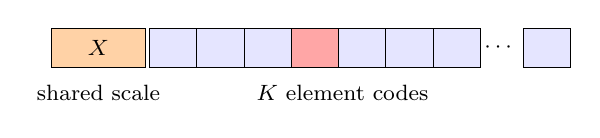
\begin{tikzpicture}[font=\footnotesize,
  cell/.style={draw, minimum width=6mm, minimum height=5mm, inner sep=0pt},
  scl/.style={draw, minimum width=12mm, minimum height=5mm, inner sep=0pt}]
  \node[scl, fill=orange!35] at (0,0) {$X$};
  \foreach \i in {1,...,7} {\node[cell, fill=blue!10] at (0.35+0.6*\i,0) {};}
  \node at (5.1,0) {$\cdots$};
  \node[cell, fill=blue!10] at (5.7,0) {};
  \node[cell, fill=red!35] at (2.75,0) {};
  \node[below=1mm] at (0,-0.25) {shared scale};
  \node[below=1mm] at (3.1,-0.25) {$K$ element codes};
\end{tikzpicture}
\par\vspace{1.4cm}
{\normalsize 7 October 2026\par}
\end{titlepage}

% =====================================================================
\pagenumbering{roman}
\section*{Abstract}
\addcontentsline{toc}{section}{Abstract}

Microscaling (MX) formats store a deep neural network's weights and activations in blocks of
$K$ narrow 4- to 8-bit elements that share one 8-bit power-of-two scale. They make
low-precision inference cheap, but they also change the fault model: a bit flip can now land
either in one element, where it corrupts one value, or in a shared scale, where it rescales all
$K$ values of the block at once. This report characterises how reliable MX networks are under
such faults.

I built \texttt{mxfi}, a bit-accurate fault-injection library that encodes tensors into real MX
bit patterns, flips bits in either fault site, and measures the effect on a network's
predictions. Using it I ran more than three million injections on ResNet8, RepVGG-A0 and a
small vision Transformer, trained on CIFAR-10 and CIFAR-100, across five element formats
(e4m3, e5m2, e3m2, e2m3, e2m1), four block sizes, weights and activations, and every bit
position. Two exhaustive campaigns, which flip every stored bit of a ResNet8, give exact
ground truth against which every sampling method is checked.

The project's core hypothesis holds on every network tested. Formats with the same accuracy
differ in fault vulnerability by up to three orders of magnitude, and the order
e3m2 $<$ e4m3 $<$ e5m2 holds on all 17 networks measured per inference. A fault in a shared
scale is always more damaging than one in an element, typically by $13\times$ to more than
$1000\times$. The dominant mechanism is the NaN and infinity codes of the 8-bit formats: on
the larger networks, the 1--8\% of element faults that land on such a code carry 97--100\% of
all element damage, no amount of model capacity absorbs them, and a simple read-side guard
that decodes them as zero cuts element damage by $29\times$ to over $4000\times$. What remains
is governed by the network's decision margins, not by its mantissa width.

The study also makes four methodological contributions. The conventional ``any image
changed'' SDC metric is shown to mostly measure whether the evaluation set contains a near-tie
input, and a per-inference rate is used instead. A margin-based severity measure predicts
failures at AUC 0.99, where the severity measure of the original problem statement performs
below chance; stratifying on it cuts the cost of a campaign by $57$--$120\times$. Single-bit
injection is shown to be sufficient, and exact enumeration of the MX code table beats learned
value intervals by two orders of magnitude.

\medskip
\noindent\textit{Keywords:} DNN reliability, microscaling, MXFP, block floating point, fault
injection, silent data corruption, shared scale, statistical fault injection.

\clearpage
\tableofcontents
\clearpage
\listoffigures
\listoftables
\clearpage
\pagenumbering{arabic}

% =====================================================================
\section{Introduction}
\label{sec:intro}

\subsection{Motivation}

Modern DNN accelerators increasingly compute in narrow number formats. Eight-bit floating
point is already common, and six- and four-bit formats are being adopted for inference. Narrow
floats have little dynamic range, so on their own they cannot represent a tensor whose values
span several orders of magnitude. The Microscaling (MX) formats standardised by the Open Compute
Project~\cite{ocp2023mx,rouhani2023mx} solve this by grouping values into blocks of $K$ (usually
32) that share one scale. Each stored value is
\[
v_i = \mathrm{decode}(c_i)\cdot 2^{X-127},
\]
where $c_i$ is a narrow element code and $X$ is the block's 8-bit E8M0 scale. The shared scale
supplies the range and the element supplies the precision, so MX formats reach close to FP32
accuracy at a fraction of the memory and bandwidth.

Hardware is not perfect. Particle strikes, voltage droop, aging and deliberate attacks such as
Rowhammer flip stored bits. In FP32 every value is a self-contained word, so a flipped bit
damages exactly one number, and decades of work on DNN fault tolerance rest on that
assumption~\cite{li2017understanding,reagen2018ares,mahmoud2020pytorchfi}. MX breaks it. A
bit flip can land in one of two structurally different places:
\begin{itemize}
\item an \emph{element code}, where it changes one value (blast radius 1); or
\item a \emph{shared scale}, where it multiplies all $K$ values of the block by
$2^{\pm 2^{j}}$ for scale bit $j$ (blast radius $K$).
\end{itemize}
Despite the rapid adoption of MX in accelerators, how these two kinds of fault behave in a
real network, and which representation choices make a network more or less vulnerable, had not
been studied. That is the gap this project addresses.

\subsection{Problem statement}

The central claim of this work is stated as a hypothesis to be tested:

\briefbox{CORE HYPOTHESIS}{Reliability of microscaling DNNs varies
substantially across formats \textbf{even at comparable inference accuracy}, and faults in the
\textbf{shared scaling factor} behave very differently from faults in individual elements,
because a single scale fault rescales an entire block of $K$ values at once.}

\noindent The study has five objectives:
\begin{enumerate}[label=\textbf{O\arabic*}]
\item \textbf{Fault propagation.} Characterise how single-bit faults in element values and in
shared scaling factors propagate through the network, and quantify the difference.
\item \textbf{Format sensitivity.} Measure fault sensitivity across MX formats (MXFP8, MXFP6,
MXFP4 and their element variants) and test whether reliability differs at comparable accuracy.
\item \textbf{Block-size effect.} Determine how block size trades efficiency against
reliability.
\item \textbf{Tensor and location.} Compare weights with activations, and fault locations
(scale versus element bit, MSB versus LSB, per layer).
\item \textbf{Vulnerability drivers.} Identify the representation characteristics (dynamic
range, exponent/mantissa split, scale granularity) that explain the observed vulnerability.
\end{enumerate}
Two design choices of the methodology are settled empirically: whether to characterise fault
impact with learned value intervals (as TreeFI~\cite{treefi2026} does for FP32) or by exact
enumeration of the MX code table, and whether single-bit injection suffices or a multi-bit
model is needed. Statistical sampling in the style of TreeFI is a supporting tool for keeping
campaigns affordable; the contribution is the reliability characterisation itself.

\subsection{Contributions}

\begin{enumerate}
\item \textbf{A bit-accurate MX fault-injection library}, \texttt{mxfi}, with both fault sites
independently addressable, exact closed-form impact tables for every (code, bit) pair, a fast
injection path for PyTorch models, and 214 unit tests (\sect{sec:method}).
\item \textbf{Exhaustive ground truth.} Two campaigns that flip every one of the $1.12$ million
stored weight bits of a ResNet8, used to validate every sampled estimate in the study
(\sect{sec:groundtruth}).
\item \textbf{A characterisation answering all five objectives}, on three architectures, two
datasets, five formats and more than sixty trained networks (\sect{sec:results}).
\item \textbf{A mechanism.} NaN/Inf element codes explain most of the difference between
formats, model capacity absorbs perturbations but never NaNs, and residual perturbation damage
follows the network's margin-normalised sensitivity (\sect{sec:drivers}).
\item \textbf{A mitigation.} A read-side guard that decodes special element codes as zero,
which removes nearly all element vulnerability of the 8-bit formats on the larger networks
(\sect{sec:guard}).
\item \textbf{Methodological corrections} for fault-injection studies in general: the
any-image SDC metric is confounded by near-tie inputs; a severity measure that works;
value-aware sampling that cuts campaign cost by $57$--$120\times$; and answers to both open
design choices (\sect{sec:methodfind}).
\item \textbf{Design guidance} for MX accelerator designers and for anyone running such
campaigns (\sect{sec:guidance}).
\end{enumerate}

\subsection{Organisation of this report}

\sect{sec:background} introduces MX formats, the fault model and the metrics.
\sect{sec:method} describes the injection library, the networks and the campaign design.
\sect{sec:results} presents the results objective by objective, followed by the NaN guard and
the CIFAR-100 replication. \sect{sec:methodfind} collects the methodological findings, and
\sect{sec:discussion} sets the results against the objectives. Design guidance, limitations
and conclusions follow. The appendices give an index of the experiments and instructions to
reproduce the results.

% =====================================================================
\section{Background}
\label{sec:background}

\subsection{Microscaling formats}

An MX tensor is split along one axis into blocks of $K$ consecutive values. Each block stores
one shared scale and $K$ element codes.

\paragraph{The shared scale.} The scale uses the E8M0 encoding: eight exponent bits and no
mantissa, so it is always an exact power of two, $2^{X-127}$ for $X\in\{0,\dots,254\}$. Code
255 is reserved for NaN. A scale therefore covers $2^{-127}$ to $2^{127}$.

\paragraph{The element formats.} Each element is a small sign--exponent--mantissa float. For a
nonzero exponent field $e$ it decodes to $(-1)^{s}(1+f/2^{M})\,2^{e-\mathrm{bias}}$, with $f$
the $M$-bit mantissa field; an all-zero exponent field gives subnormals. \tab{tab:formats}
lists the five formats studied. The property that turns out to matter most is in the last
column: only the two 8-bit formats reserve bit patterns for NaN or infinity.

\begin{table}[htbp]
\centering\small
\caption{MX element formats. The two 8-bit formats reserve codes for NaN or infinity. The 6-
and 4-bit formats do not, so every one of their bit patterns is a finite number.}
\label{tab:formats}
\begin{tabular}{llcccc}
\toprule
format & family & sign/exp./mantissa bits & bias & largest value & NaN/Inf codes \\
\midrule
e4m3 & MXFP8 & 1/4/3 & 7  & 448      & 2 (NaN) \\
e5m2 & MXFP8 & 1/5/2 & 15 & 57{,}344 & 8 (2 Inf, 6 NaN) \\
e3m2 & MXFP6 & 1/3/2 & 3  & 28       & none \\
e2m3 & MXFP6 & 1/2/3 & 1  & 7.5      & none \\
e2m1 & MXFP4 & 1/2/1 & 1  & 6        & none \\
\bottomrule
\end{tabular}
\end{table}

\fig{fig:alphabets} draws every positive value each format can hold. The wide-exponent formats
cover a huge range, but in MX the shared scale already supplies the range, so most of that
reach goes unused: after scaling, a block's values occupy only the top few binades of the
element format. This is why e5m2 and e3m2, which share a 2-bit mantissa, quantise real weights
almost identically despite their very different exponent widths.

\begin{figure}[htbp]
\centering
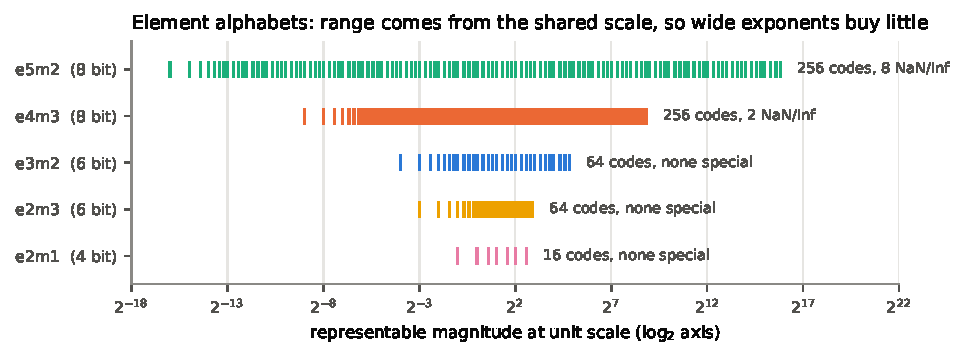
\includegraphics[width=\linewidth]{figures/fig5_alphabets.pdf}
\caption{Every finite positive value of each element format at unit scale. Each tick is one
code. The 8-bit formats spend their extra codes on range the shared scale already provides,
and reserve some codes for NaN and infinity.}
\label{fig:alphabets}
\end{figure}

\subsection{Choosing the shared scale}

The OCP specification chooses each block's scale so that the largest magnitude in the block
lands in the top binade of the element format:
\[
X - 127 = \big\lfloor \log_2 \max_i |v_i| \big\rfloor - e_{\max},
\]
where $e_{\max}=\lfloor\log_2(\text{largest element value})\rfloor$. Because the largest
representable element sits below the top of that binade, the block maximum can be clipped.

\paragraph{Worked example.} For e4m3, $e_{\max}=\lfloor\log_2 448\rfloor=8$, so the top binade
is $[256,512)$ but the format stops at 448, a headroom of $87.5\%$. A block whose largest value
is $3.7$ gets $X-127=1-8=-7$, a scale of $1/128$. Then $3.7\times128=473.6$, which exceeds 448
and saturates: the block maximum is clipped by about 5\%. In the worst case the clip is
$12.5\%$ for e4m3, e5m2 and e3m2, $6.25\%$ for e2m3 and $25\%$ for e2m1.

Since clipping could confound a comparison between formats, I also implemented a non-clipping
rule, which I call \emph{fit}: the smallest scale at which the block maximum is representable,
$X-127=\lceil\log_2(\max_i|v_i|/\text{largest element})\rceil$. All results use the OCP rule
unless stated otherwise; the fit rule is a control.

\subsection{The two fault sites}

\fig{fig:block} shows one block and its two fault sites.

\begin{itemize}
\item An \textbf{element fault} flips bit $b$ of one code. A mantissa bit nudges the value, an
exponent bit multiplies it by a power of two, and the sign bit negates it. In e4m3 and e5m2 a
flip can also turn the code into NaN or infinity.
\item A \textbf{scale fault} flips bit $j$ of $X$. If the bit was 0 the exponent rises by $2^j$;
if it was 1 the exponent falls by $2^j$. All $K$ values are multiplied by $2^{\pm2^j}$ at
once. Flipping bit 7 shifts the exponent by 128, beyond the range of float32, so the block
overflows to infinity. Reaching code 255 turns the whole block into NaN.
\end{itemize}

\begin{figure}[htbp]
\centering
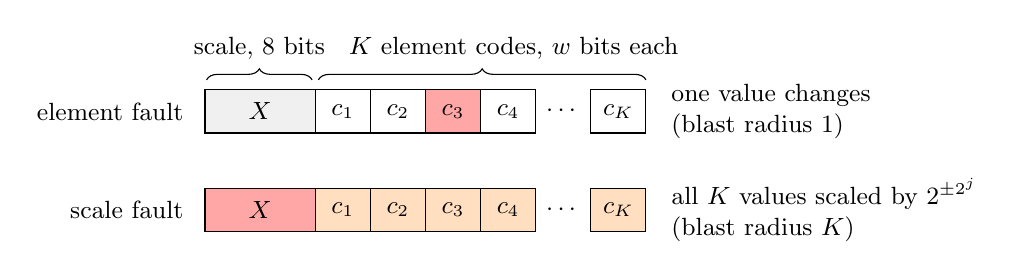
\begin{tikzpicture}[font=\small,
  cell/.style={draw, minimum width=7mm, minimum height=5.5mm, inner sep=0pt},
  scl/.style={draw, minimum width=14mm, minimum height=5.5mm, inner sep=0pt}]
  \node[anchor=east] at (-0.15,0) {element fault};
  \node[scl, fill=gray!12] at (0.7,0) {$X$};
  \node[cell] at (1.75,0) {$c_1$};
  \node[cell] at (2.45,0) {$c_2$};
  \node[cell, fill=red!35] at (3.15,0) {$c_3$};
  \node[cell] at (3.85,0) {$c_4$};
  \node at (4.55,0) {$\cdots$};
  \node[cell] at (5.25,0) {$c_K$};
  \node[anchor=west, align=left] at (5.8,0) {one value changes\\(blast radius 1)};
  \node[anchor=east] at (-0.15,-1.25) {scale fault};
  \node[scl, fill=red!35] at (0.7,-1.25) {$X$};
  \foreach \x/\n in {1.75/1,2.45/2,3.15/3,3.85/4} {\node[cell, fill=orange!25] at (\x,-1.25) {$c_\n$};}
  \node at (4.55,-1.25) {$\cdots$};
  \node[cell, fill=orange!25] at (5.25,-1.25) {$c_K$};
  \node[anchor=west, align=left] at (5.8,-1.25) {all $K$ values scaled by $2^{\pm2^{j}}$\\(blast radius $K$)};
  \draw[decorate, decoration={brace, amplitude=4pt}] (0.02,0.4) -- (1.36,0.4)
    node[midway, above=4pt] {scale, 8 bits};
  \draw[decorate, decoration={brace, amplitude=4pt}] (1.44,0.4) -- (5.6,0.4)
    node[midway, above=4pt, xshift=4mm] {$K$ element codes, $w$ bits each};
\end{tikzpicture}
\caption{One MX block and its two fault sites. Red marks the flipped word and orange the
values it alters.}
\label{fig:block}
\end{figure}

A short calculation already suggests the scale will matter. A block occupies $8+Kw$ bits, of
which only 8 belong to the scale: about 3\% for $K=32$ and $w=8$. If every stored bit is
equally likely to flip, the expected number of corrupted \emph{values} per block is $8K$ from
scale faults and $Kw$ from element faults, a ratio of $8:w$. An 8-bit format therefore receives
about half of its corrupted values through the 3\% of storage that holds scales, and a 4-bit
format about two thirds.

\subsection{Fault model}

The study adopts the single-bit flip, standard in DNN fault-injection studies, generalised to
both MX sites and to weights and activations. It models fault \emph{occurrence} separately from
fault \emph{impact}. Occurrence is a per-bit-position flip rate
$\pi_{\mathrm{site},b}=\pi^0_{\mathrm{site}}\kappa_{\mathrm{site}}(b)$, where $\kappa$ is a
susceptibility profile with mean 1. A pattern $S$ of simultaneously flipped bits in one word
has the Poisson--binomial probability
\[
P(S)=\prod_{b\in S}\pi_b\prod_{b\notin S}(1-\pi_b),\qquad
H=1-\prod_b(1-\pi_b)\approx\sum_b\pi_b+\sum_{b<b'}\pi_b\pi_{b'}+O(\pi^3),
\]
where $H$ is the word-corruption rate. The single-bit term is the baseline and the multi-bit
tail an optional extension (\sect{sec:multibit} shows it is not needed). A natural severity
for an element fault is the log-ratio $d=|\log v'-\log v|$, and for a scale fault
$D_s=K|X'-X|\log 2$. \sect{sec:severity} shows that $d$ does not predict failure and gives a
measure that does.

\subsection{Metrics}
\label{sec:metrics}

Let $D$ be a fixed evaluation set of $N$ images, $\hat y_i$ the prediction of the fault-free,
MX-quantised network (the \emph{golden} prediction) and $\hat y_i^{\varphi}$ the prediction
under fault $\varphi$. For a set $\Phi$ of injected faults I use two rates:
\begin{align*}
\text{any-image SDC rate} &= \frac{1}{|\Phi|}\sum_{\varphi\in\Phi}
  \mathbf{1}\Big[\exists\, i:\ \hat y_i^{\varphi}\ne\hat y_i\Big],\\
\text{per-inference rate} &= \frac{1}{|\Phi|}\sum_{\varphi\in\Phi}
  \frac{1}{N}\sum_{i=1}^{N}\mathbf{1}\Big[\hat y_i^{\varphi}\ne\hat y_i\Big].
\end{align*}
The any-image rate is the conventional silent-data-corruption (SDC) metric. The per-inference
rate answers the question a system designer actually asks: given one fault, how likely is a
particular inference to be wrong? A network output containing NaN or infinity counts as a
changed prediction for every affected image, and I also track the \emph{non-finite rate}, the
fraction of faults that produce a non-finite output.

\sect{sec:metricfind} shows that the any-image rate mostly measures the evaluation set rather
than the fault, so the per-inference rate is the primary metric. \textbf{All rates in this
report are per inference unless stated otherwise.} Proportions carry Wilson 95\% intervals~\cite{wilson1927}; per-inference rates carry
normal intervals on the mean over faults, or bootstrap intervals over images where noted.

\subsection{Related work}

Fault-injection studies have shown that errors in DNNs propagate differently by layer, data
type and bit position~\cite{li2017understanding}. Tools such as Ares~\cite{reagen2018ares} and
PyTorchFI~\cite{mahmoud2020pytorchfi} made such campaigns routine for FP32 and integer models,
and bit-flip attacks~\cite{hong2019terminal,rakin2019bfa} show how few flips it can take to
destroy accuracy. Statistical fault injection bounds the error of a sampled
campaign~\cite{leveugle2009sfi}. TreeFI~\cite{treefi2026} reduces the cost of such campaigns
for FP32 by learning value intervals with similar bit-flip behaviour and stratifying over them.
None of these models a shared scale, which is the gap this work addresses. The MX formats
themselves are described in~\cite{rouhani2023mx,ocp2023mx}.

% =====================================================================
\section{Methodology}
\label{sec:method}

\subsection{The \texttt{mxfi} fault-injection library}

\texttt{mxfi} is a fault-injection library written for this study. Its core is plain \texttt{numpy} with no deep-learning
dependency, so the bit-level logic can be tested in isolation; a separate layer connects it to
PyTorch models. \tab{tab:modules} lists its modules.

\begin{table}[htbp]
\centering\small
\caption{Modules of the \texttt{mxfi} library (about 2{,}300 lines).}
\label{tab:modules}
\begin{tabular}{@{}lL{0.70\linewidth}@{}}
\toprule
module & role \\
\midrule
\texttt{formats} & Exact lookup table of every code of every element format; E8M0 encode/decode. \\
\texttt{codec} & \texttt{quantize()} to an \texttt{MXTensor} with separately addressable
\texttt{scales} and \texttt{codes} arrays; OCP and fit scale rules; round-to-nearest-even with
saturation; padding of partial blocks. \\
\texttt{faults} & \texttt{Fault(site, index, bit)} and \texttt{inject()}; exact impact tables
for every (code, bit) element flip and every (byte, bit) scale flip. \\
\texttt{torch\_mx} & Wraps a PyTorch model so its weights (and optionally activations) carry MX
values; fast single-fault injection and restoration; multi-bit word faults. \\
\texttt{sampling} & Uniform and stratified fault sampling with inclusion weights; Neyman and
proportional allocation. \\
\texttt{stats} & Wilson intervals, the stratified estimator, injection-reduction factors. \\
\texttt{campaign} & Golden-versus-faulty campaign driver; one row per fault with outcome and
predicted severity. \\
\texttt{models}, \texttt{vit}, \texttt{data}, \texttt{train} & ResNet8, RepVGG-A0 and the ViT;
batch-norm folding and branch fusion; CIFAR loaders and fixed evaluation subsets; training. \\
\bottomrule
\end{tabular}
\end{table}

\paragraph{Code-domain injection.} Tensors are encoded into real MX bit patterns and the fault
is applied to the stored code before decoding. This is what lets a scale fault perturb all $K$
values and lets an element fault land on a NaN code. The codec stores the two sites as
separate \texttt{uint8} arrays, \texttt{scales[..., n\_blocks]} and
\texttt{codes[..., n\_blocks, K]}, and a fault is an XOR of \texttt{1 << bit} into one of
them. Lanes that only pad a partial final block are excluded from every campaign, since they
hold no model value.

\paragraph{Exact impact tables.} An element alphabet has at most 256 codes, so the decoded
value before and after every (code, bit) flip can be tabulated in closed form,
$|v'-v|=|\mathrm{table}[c\oplus2^b]-\mathrm{table}[c]|\cdot2^{X-127}$, together with flags for
sign flips and for flips into or out of a special code. The scale table does the same for all
$256\times8$ scale flips. These tables cost nothing to compute and became the basis of the
value-aware sampling in \sect{sec:sampling}.

\paragraph{Deployment form.} Batch normalisation is folded into the preceding convolution, and
RepVGG's branches are fused into single $3\times3$ convolutions, before quantisation. An
unfolded batch norm would re-normalise whatever a corrupted convolution produced and hide part
of the damage; deployed accelerators fold it. Weights are blocked along the reduction axis,
the way MX hardware reads them: a linear weight $(\mathit{out},\mathit{in})$ along
$\mathit{in}$, and a convolution weight viewed as $(\mathit{out},\mathit{in}\cdot k_h\cdot
k_w)$. Activations are blocked along channels for convolutions and features for linear layers.
LayerNorm in the ViT is left unquantised, as in deployment.

\paragraph{Fast injection.} Rebuilding a whole layer for every fault would be slow. The fast
path computes which weights a fault touches (one for an element fault, $K$ for a scale fault)
and their new values, writes just those into the live weight tensor, runs the network, and
restores them. A reference path that re-encodes the whole tensor is kept, and a check confirms
that both give identical outputs. On an A100 the fast path reaches about 170 injections per
second on 200 images.

\paragraph{NaN semantics.} Following the OCP conversion, a NaN anywhere in a block makes the
block maximum NaN, hence the scale NaN, hence the whole block NaN. This matters for activation faults: an
activation-quantised layer re-encodes its input, and a codec that mapped NaN to zero would
silently erase a NaN created by an activation fault at the next layer. A unit test pins the
behaviour.

\paragraph{Verification.} The library has 214 unit tests (codec round trips, exact alphabets,
fault tables, sampling weights, the PyTorch pipeline), all passing. Two tools check
experiments rather than code: one confirms that the fast and reference injection paths agree,
and one replays a sample of a recorded campaign's faults against a checkpoint to confirm that
the campaign was produced by that exact network (\sect{sec:provenance}).

\subsection{Networks and training}

\tab{tab:models} summarises the networks. ResNet8 is the MLPerf Tiny image
classifier~\cite{banbury2021mlperftiny,he2016resnet}. To isolate model capacity I also trained
it at five base widths (8 to 48 channels), a $35\times$ range of parameter counts. RepVGG-A0
\cite{ding2021repvgg} is a plain re-parameterisable CNN. The ViT keeps the width (192) and head
count (3) of DeiT-Tiny~\cite{touvron2021deit} at depth 6 with $4\times4$ patches, a size
suited to $32\times32$ images~\cite{dosovitskiy2021vit}. CNNs were trained with SGD (Nesterov
momentum 0.9, learning rate 0.1, weight decay $10^{-4}$, cosine schedule); the ViT with AdamW
(learning rate $10^{-3}$, weight decay 0.05, label smoothing 0.1). Standard random-crop and
flip augmentation was used throughout.

\begin{table}[htbp]
\centering\small
\caption{Networks used in the study. Accuracies are FP32 top-1 on the full test set; seeds
count independently trained networks used in campaigns.}
\label{tab:models}
\begin{tabular}{lrrcccc}
\toprule
network & parameters & epochs & CIFAR-10 & seeds & CIFAR-100 & seeds \\
\midrule
ResNet8 (reference)  & 78\,K   & 60  & 87.0\%       & 1   & 58\%     & 3 \\
ResNet8, widths 8--48 & 20--692\,K & 30 & 80.0--89.6\% & up to 10 & -- & -- \\
RepVGG-A0 (fused)    & 7.0\,M  & 30  & 91.4\%       & 3   & 70--71\% & 3 \\
ViT (DeiT-Tiny width) & 2.7\,M & 100 & 80.4--81.9\% & 3   & 47--49\% & 3 \\
\bottomrule
\end{tabular}
\end{table}

\begin{figure}[htbp]
\centering
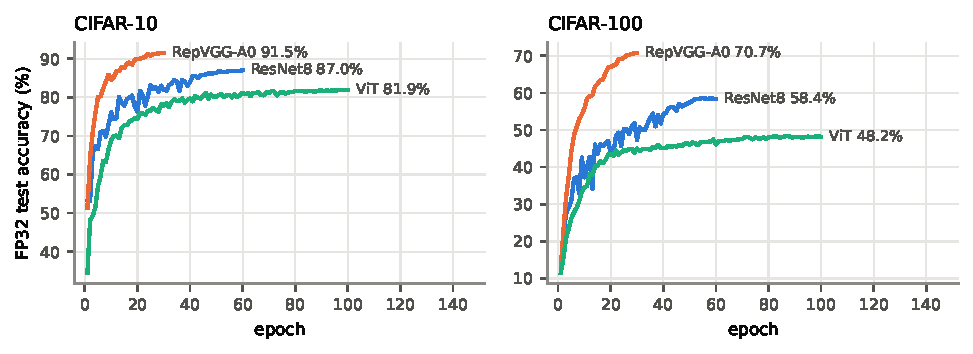
\includegraphics[width=\linewidth]{figures/fig6_training.pdf}
\caption{Test accuracy during training for the seed-0 network of each architecture.}
\label{fig:training}
\end{figure}

\fig{fig:accuracy} shows the accuracy after MX quantisation at $K=32$. On every network the
6- and 8-bit formats sit within about a point of each other, and on the ViT within $0.2$ points
of FP32, so reliability can be compared at matched accuracy, which is what the core hypothesis
requires. MXFP4 (e2m1) loses several points on the CNNs, mostly through OCP clipping: on
RepVGG the fit rule recovers $7.9$ points.

\begin{figure}[htbp]
\centering
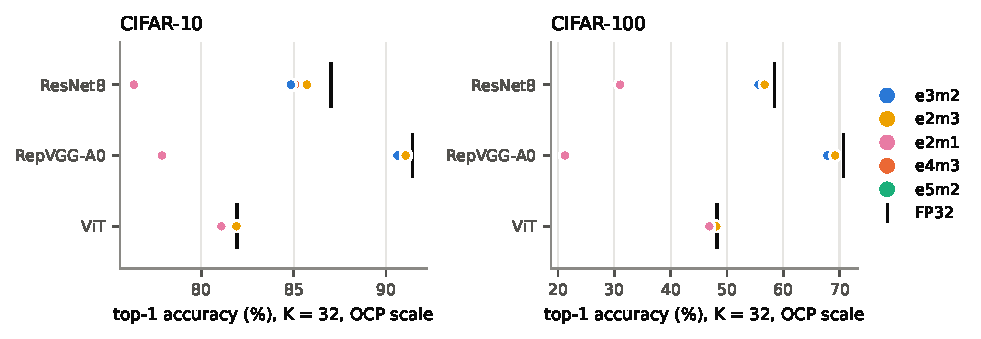
\includegraphics[width=\linewidth]{figures/fig7_accuracy.pdf}
\caption{Top-1 accuracy after MX quantisation of all weights ($K=32$, OCP scale rule) against
the FP32 baseline (black tick). The 6- and 8-bit formats are matched in accuracy on every
network; MXFP4 is the outlier on the CNNs.}
\label{fig:accuracy}
\end{figure}

\subsection{Campaign design}

Algorithm~\ref{alg:campaign} shows a weight campaign. Each fault is scored on a fixed,
class-balanced subset of 200 test images (2 per class on CIFAR-100), materialised once so that
every injection replays byte-identical inputs and any difference is attributable to the fault
alone. A campaign records, for each fault, its location, which predictions changed, whether the
output went non-finite, and the severity the exact tables predicted for it.

\begin{algorithm}[htbp]
\small
\caption{Weight fault-injection campaign in \texttt{mxfi}}
\label{alg:campaign}
\begin{algorithmic}[1]
\Require network $M$, format $F$, block size $K$, evaluation set $D$, budget $n$
\State $M\gets\textsc{Deploy}(M)$ \Comment{fold batch norm, fuse branches}
\ForAll{quantisable layers $\ell$}
  \State view $W_\ell$ as (outputs $\times$ reduction); split the reduction axis into blocks of $K$
  \State $X_\ell\gets$ per-block scale (OCP rule);\; $C_\ell\gets\mathrm{round}_F(W_\ell\, 2^{-X_\ell})$
  \State $W_\ell\gets\textsc{Decode}(X_\ell,C_\ell)$ \Comment{the network now holds MX values}
\EndFor
\State $\hat y\gets\arg\max M(D)$ \Comment{golden predictions}
\For{$t=1$ to $n$}
  \State draw $\varphi=(\ell,\mathrm{site},\mathrm{index},b)$ uniformly over all stored bits
  \If{site $=$ element} $C_\ell[\mathrm{index}]\gets C_\ell[\mathrm{index}]\oplus 2^{b}$; re-decode that one weight
  \Else{}\; $X_\ell[\mathrm{index}]\gets X_\ell[\mathrm{index}]\oplus 2^{b}$; re-decode the $K$ weights of the block
  \EndIf
  \State $\hat y^{\varphi}\gets\arg\max M(D)$; record which images changed and non-finiteness; restore
\EndFor
\State \Return rates over all faults with confidence intervals
\end{algorithmic}
\end{algorithm}

\noindent Most campaigns draw 3000 faults uniformly over every stored bit, which is the
physically faithful model for a uniform per-bit upset rate. Replacing the sampling step with an
enumeration of every stored bit makes a campaign \emph{exhaustive}. Activation faults go through
forward hooks that quantise a layer's input to MX, flip one bit of one image's encoding, and
decode; since activation blocks never span images, this is the exact per-inference fault
space. A weight fault is persistent and is read by every inference until the word is
rewritten; an activation fault is transient and affects one inference.

\paragraph{Stratified sampling.} When a stratum matters more than its share of storage, faults
are drawn per stratum with inclusion weights $w_h=W_h/n_h$, where $W_h$ is the stratum's share
of the bit population and $n_h$ its number of draws, so the weighted mean stays an unbiased
estimate of the model-wide rate. Allocation follows Neyman's rule~\cite{neyman1934},
$n_h\propto W_h\sigma_h$, with an optional blast-radius weight $\Phi$ for scale
strata. For a proportion $\sigma_h=\sqrt{p_h(1-p_h)}$; for the per-inference rate, which is a
mean rather than a proportion, $\sigma_h$ is estimated from a pilot.

\subsection{Exhaustive ground truth and validation}
\label{sec:groundtruth}

On ResNet8 (width 16) I flipped every one of the $638{,}624$ stored weight bits under e4m3 and
all $483{,}904$ under e3m2, scoring each on the 200 images. Each took about an hour on an A100.
These two campaigns give the exact rates, with no sampling error, against which the sampled
campaigns and every sampling method were checked (\tab{tab:validation}).

\begin{table}[htbp]
\centering\small
\caption{A 3000-fault uniform campaign against exhaustive truth (ResNet8, e4m3, any-image
rate). The sampled interval covers the truth.}
\label{tab:validation}
\begin{tabular}{lc}
\toprule
exhaustive truth ($638{,}624$ faults) & $0.4171$ \\
uniform estimate, $n=3000$ & $0.4270$ \\
95\% Wilson interval & $[0.4094,\ 0.4448]$ \\
relative error & $2.4\%$ \\
\bottomrule
\end{tabular}
\end{table}

\subsection{Checkpoint provenance}
\label{sec:provenance}

Training is not bit-reproducible across machines: networks trained from the same seed on a CPU
and on a GPU reach the same accuracy to a few tenths of a percent but hold different weights.
A campaign analysed against the wrong copy would silently pair outcomes with the wrong network.
Every analysis therefore runs a replay check, which re-injects a sample of a campaign's
recorded faults into the checkpoint and requires identical outcomes. The two exhaustive
campaigns were recorded on two independently trained networks; they serve as two independent
references and are never used as a comparison between formats.

\subsection{Scale of the study}

In total the study ran about $1.44$ million sampled weight injections in 119 campaigns on
CIFAR-10, the two exhaustive campaigns ($1.12$ million), $390{,}000$ multi-bit injections, and
further campaigns for activations, the NaN guard and CIFAR-100, on more than sixty
independently trained networks. Experiments ran on a 4-core CPU (47\,ms per injection on 100
images) and on two NVIDIA A100 GPUs at IIT Kanpur.

% =====================================================================
\section{Results}
\label{sec:results}

The results are organised by objective. O2 comes first because it states the core
hypothesis.

\subsection{O2: Equal accuracy, very different reliability}
\label{sec:formats}

\fig{fig:accvuln} puts accuracy and fault vulnerability side by side. Within about one point of
accuracy, the per-inference damage of an element fault spans more than two orders of magnitude
on ResNet8 and nearly four on RepVGG and the ViT. On the ViT, e5m2 and e3m2 differ by $0.01$
points of accuracy, yet a single e5m2 element fault is about $2000$ times as likely as an e3m2
one to corrupt a given inference.

\begin{figure}[htbp]
\centering
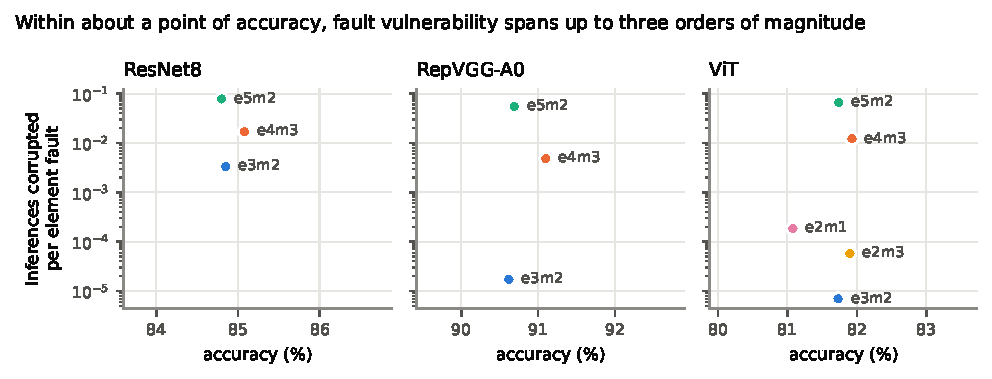
\includegraphics[width=\linewidth]{figures/fig8_acc_vs_vuln.pdf}
\caption{Quantised accuracy against per-inference damage of an element fault (seed-0 networks,
CIFAR-10, $K=32$). Each point is one format; vulnerability is on a log scale.}
\label{fig:accvuln}
\end{figure}

\fig{fig:formatorder} and \tab{tab:formats-result} show that the ordering is consistent.
e3m2 $<$ e4m3 $<$ e5m2 holds on every CIFAR-10 configuration, with disjoint 95\% intervals
between all three formats on every row, and on all nine CIFAR-100 networks.

\keybox{Formats of equal accuracy differ in fault vulnerability by up to three orders of
magnitude. Measured per inference, e3m2 $<$ e4m3 $<$ e5m2 on all 8 CIFAR-10 configurations and
all 9 CIFAR-100 networks. Accuracy is not a reliability proxy.}

\begin{figure}[htbp]
\centering
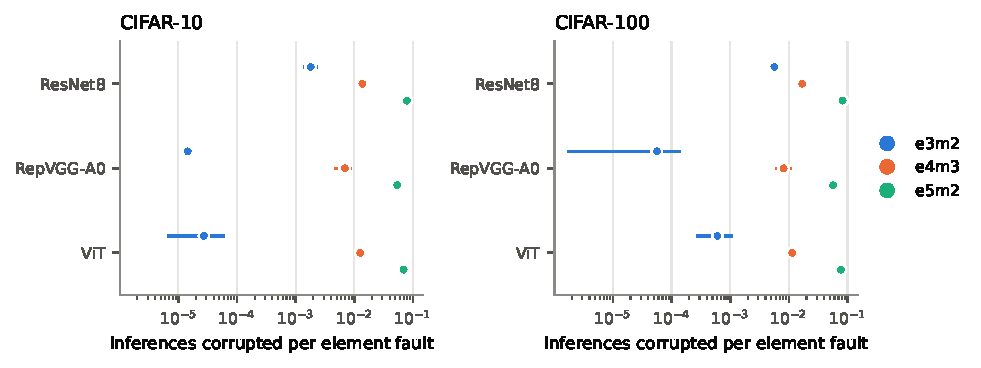
\includegraphics[width=\linewidth]{figures/fig9_format_order.pdf}
\caption{Per-inference damage of an element fault by format, mean over seeds with the range
across seeds (ResNet8 width 16: 5 seeds on CIFAR-10, 3 on CIFAR-100; others 3 seeds each).}
\label{fig:formatorder}
\end{figure}

\begin{table}[htbp]
\centering\small
\caption{Per-inference rate of element faults, CIFAR-10, $K=32$, averaged over seeds. Lower is
better.}
\label{tab:formats-result}
\begin{tabular}{lcccc}
\toprule
network & seeds & e3m2 (6-bit) & e4m3 (8-bit) & e5m2 (8-bit) \\
\midrule
RepVGG-A0     & 3 & 0.00001 & 0.00688 & 0.05381 \\
ViT           & 3 & 0.00003 & 0.01258 & 0.06897 \\
ResNet8 (reference) & 1 & 0.00332 & 0.01699 & 0.07801 \\
ResNet8, width 8  & 5 & 0.01003 & 0.02005 & 0.08143 \\
ResNet8, width 16 & 5 & 0.00180 & 0.01374 & 0.07831 \\
ResNet8, width 24 & 4 & 0.00121 & 0.01210 & 0.07585 \\
ResNet8, width 32 & 4 & 0.00060 & 0.01354 & 0.07934 \\
ResNet8, width 48 & 4 & 0.00035 & 0.01302 & 0.07812 \\
\bottomrule
\end{tabular}
\end{table}

The failure \emph{mode} differs as well as the rate. e5m2 has eight special codes and a wide
exponent; on ResNet8 $7.7\%$ of its weight faults produced a non-finite output. e3m2 has no
special codes and can never produce a non-finite value from an element flip. Why the formats
are ordered this way is the subject of \sect{sec:drivers}.

\subsection{O1: Shared-scale faults versus element faults}
\label{sec:sites}

\fig{fig:sites} compares the two sites on every network and format. A scale fault is more
damaging than an element fault in every one of the 18 cells, by $1.7\times$ to $8400\times$.
The ratio is smallest for e5m2, whose element faults already corrupt many inferences through
the NaN pathway, and largest for e3m2 on the larger networks, whose element faults almost never
matter. The largest ratios divide by an element rate that is statistically close to zero and
should be read as lower bounds of order $10^3$.

\begin{figure}[htbp]
\centering
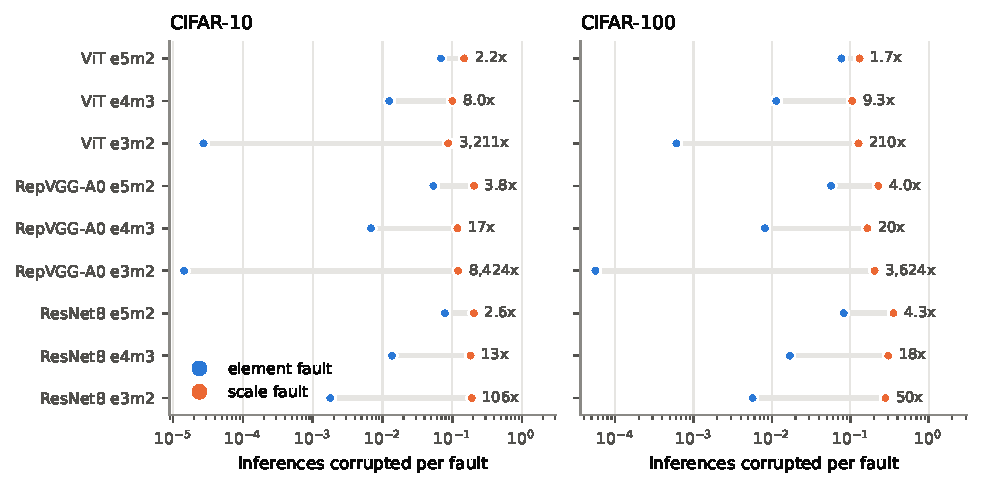
\includegraphics[width=\linewidth]{figures/fig10_scale_vs_element.pdf}
\caption{Per-inference damage of an element fault (blue) and a scale fault (orange), with the
ratio between them, for every network and format. Mean over seeds.}
\label{fig:sites}
\end{figure}

The exhaustive campaigns give exact numbers (\tab{tab:exact-sites}). Under e3m2, the scale bytes
are $4.1\%$ of storage but carry $87.6\%$ of all fault damage; under e4m3 they are $3.1\%$ of
storage and carry $32.7\%$. $94.4\%$ of all possible e4m3 scale flips change at least one
prediction, and $12.3\%$ produce a non-finite output, for every format, since the E8M0 scale has
its own NaN code and its top bit is worth 128 exponent steps.

\begin{table}[htbp]
\centering\small
\caption{Exact site asymmetry from the two exhaustive campaigns (ResNet8, $K=32$). The two
campaigns used different trained networks, so compare sites within a column, not formats
across columns.}
\label{tab:exact-sites}
\begin{tabular}{lcc}
\toprule
 & e4m3 & e3m2 \\
\midrule
faults (element / scale) & $618{,}880$ / $19{,}744$ & $464{,}160$ / $19{,}744$ \\
element fault, per-inference rate & 0.01635 & 0.00113 \\
scale fault, per-inference rate & 0.24943 & 0.18865 \\
scale / element & $15.3\times$ & $166\times$ \\
scale share of storage & 3.1\% & 4.1\% \\
scale share of all damage & 32.7\% & 87.6\% \\
scale faults with non-finite output & 12.3\% & 12.3\% \\
\bottomrule
\end{tabular}
\end{table}

\paragraph{Which scale bits matter.} On this network the scale bytes lie between 114 and 120,
so bits 4--6 are always set and bit 3 almost never. Flipping bit 3 raises the exponent by 8 and
multiplies the block by 256, corrupting $75\%$ of inferences; flipping bit 7 overflows the block
($98\%$). Flipping bits 4--6 lowers the exponent and shrinks the block towards zero, corrupting
only $3\%$ (\fig{fig:perbit}, right). Growing a block is catastrophic; shrinking it is mild. Not
one of the $2{,}468$ flips of bit 3 or bit 7 left the predictions intact.

\keybox{A scale fault is always more damaging than an element fault, typically by $13\times$ to
more than $1000\times$, on every architecture, format, tensor type and dataset. Scale bits are
2--11\% of storage but can carry most of the damage. The scale flips that grow a block are the
dangerous ones.}

\subsection{O3: Block size}
\label{sec:blocksize}

Block size changes three things at once (\fig{fig:blocksize}). Larger blocks shrink the share of
storage taken by scales from $11.1\%$ at $K=8$ to $1.7\%$ at $K=64$, so a scale is less likely
to be hit. Each scale fault becomes worse, because it rescales more values. And element faults
become milder: a larger block has a larger maximum, so typical values sit further below the
shared scale and a flipped bit moves them less in absolute terms. Accuracy moves by less than
about one point across $K$, so this axis carries no accuracy confound.

\begin{figure}[htbp]
\centering
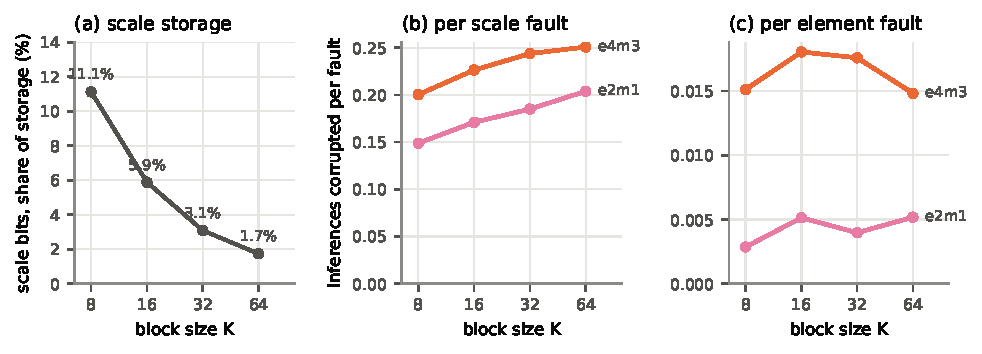
\includegraphics[width=\linewidth]{figures/fig11_block_size.pdf}
\caption{Block size on ResNet8. (a) The scale's share of storage. (b) Per-inference damage of a
scale fault, which grows with $K$. (c) Per-inference damage of an element fault, which mostly
falls with $K$ for e4m3.}
\label{fig:blocksize}
\end{figure}

Because OCP clipping changes with $K$, the element-side trend could in principle be an artefact
of the scale rule. A matched-fault experiment (one fixed set of weight positions and bits
injected at every $K$) rules this out: a monotone trend appears under \emph{both} the OCP and
the non-clipping rule (\fig{fig:blockrule}). Under the any-image metric the OCP rule exaggerates
the trend, a further instance of the metric problem of \sect{sec:metricfind}.

\begin{figure}[htbp]
\centering
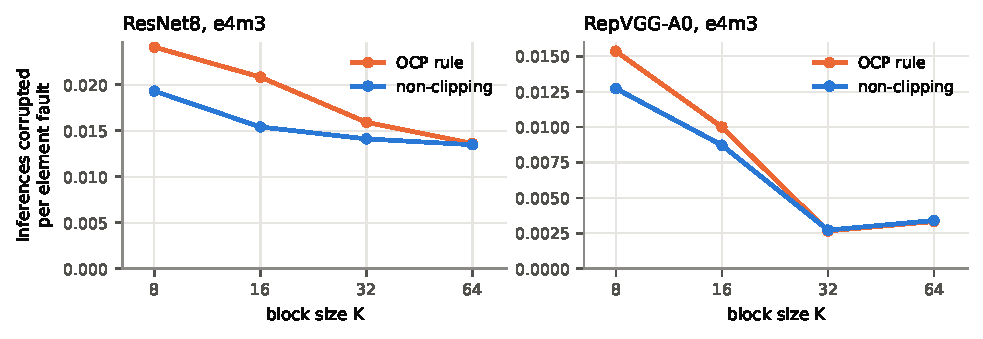
\includegraphics[width=\linewidth]{figures/fig12_block_rule.pdf}
\caption{Matched element faults across block sizes under the OCP and the non-clipping scale
rule (e4m3, per inference). The trend is present under both rules.}
\label{fig:blockrule}
\end{figure}

\keybox{Block size is a genuine trade-off, with the two fault sites moving in opposite
directions: larger blocks make scale faults rarer but worse, and element faults milder. With
protected scales, large blocks are safe.}

\subsection{O4: Tensor type and fault location}
\label{sec:location}

\paragraph{Bit position.} \fig{fig:perbit} gives the exact damage of every bit position from
the e4m3 exhaustive campaign, split by whether the output stayed finite. Among faults that leave
the output finite, the sign bit is the most damaging element bit. In total damage it ranks
seventh of eight. The $1.27\%$ of element faults that flip a code into the NaN pattern
\texttt{S.1111.111} each corrupt every inference, and together they carry $77.6\%$ of all
element damage. A sign flip never touches the magnitude bits, so it is the one flip that can
never reach the NaN code. In e3m2, which has no NaN code, the sign bit is simply the worst bit.

\begin{figure}[htbp]
\centering
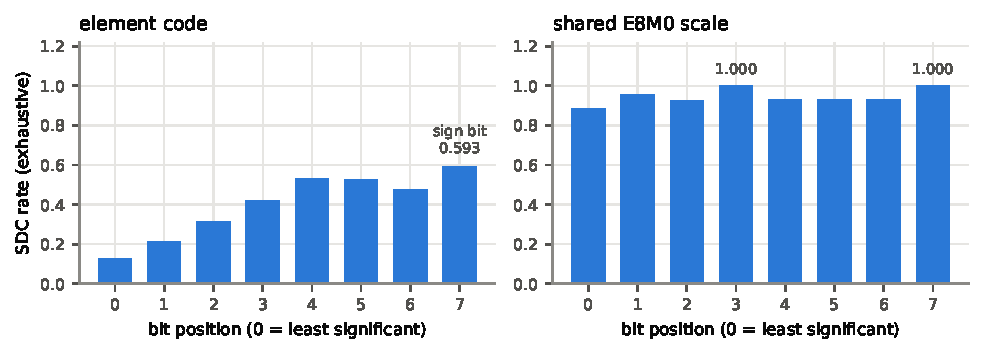
\includegraphics[width=\linewidth]{figures/fig1_per_bit.pdf}
\caption{Exhaustive per-bit damage per inference (ResNet8, e4m3, $K=32$, $638{,}624$
injections), split by whether the output stayed finite. The sign bit does the most finite
damage, but most element damage comes from flips into the NaN code. Scale bits 3 and 7 are
almost never set, so flipping them grows the block $256\times$ or overflows it.}
\label{fig:perbit}
\end{figure}

\paragraph{Layer.} Vulnerability runs \emph{opposite} to layer size (\fig{fig:layers}). The
3584-bit stem convolution is the most fragile layer, because its errors propagate through the
whole network; the $304{,}128$-bit final convolution is the most robust. A uniform campaign
samples layers in proportion to size, so it spends $48\%$ of its budget on the most robust layer
and $0.6\%$ on the most fragile.

\begin{figure}[htbp]
\centering
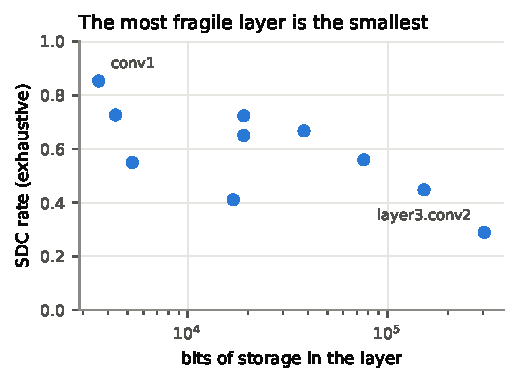
\includegraphics[width=0.55\linewidth]{figures/fig3_layers.pdf}
\caption{Exhaustive any-image SDC rate of each ResNet8 layer against its storage (e4m3). The
smallest layer, the stem, is the most fragile.}
\label{fig:layers}
\end{figure}

\paragraph{Weights versus activations.}
\label{sec:act}
Weights and activations must be compared per inference, since a weight fault is exposed to every
inference and an activation fault to one. Measured that way, an element fault in a weight does $0.3$--$2.2\times$ the damage of one in an activation,
and at the scale site $0.9$--$1.7\times$ (\fig{fig:act}, \tab{tab:act}). Under e4m3 on CIFAR-10
the two are statistically indistinguishable. The reason is the same in both tensors: about 1\%
of faults land on a special code and destroy the inference. The real difference between weights
and activations is \emph{exposure}: how long a word is resident and how often it is read.

\begin{figure}[htbp]
\centering
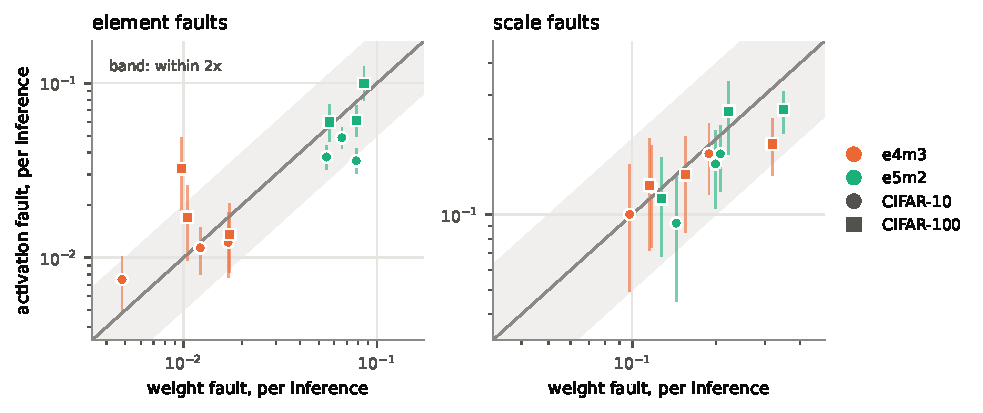
\includegraphics[width=\linewidth]{figures/fig19_activations.pdf}
\caption{Per-inference damage of a fault in a weight against one in an activation, with 95\%
bootstrap intervals for activations. Points inside the grey band are within a factor of 2.}
\label{fig:act}
\end{figure}

\begin{table}[htbp]
\centering\small
\caption{Per-inference rate of element faults in weights and activations (CIFAR-10, $K=32$).}
\label{tab:act}
\begin{tabular}{llccc}
\toprule
network & format & weight & activation [95\% CI] & weight / activation \\
\midrule
ResNet8   & e4m3 & 0.0170 & 0.0122 [0.0077, 0.0182] & $1.4\times$ \\
RepVGG-A0 & e4m3 & 0.0048 & 0.0075 [0.0049, 0.0101] & $0.64\times$ \\
ViT       & e4m3 & 0.0122 & 0.0114 [0.0080, 0.0150] & $1.07\times$ \\
ResNet8   & e5m2 & 0.0780 & 0.0359 [0.0302, 0.0421] & $2.2\times$ \\
RepVGG-A0 & e5m2 & 0.0549 & 0.0378 [0.0319, 0.0442] & $1.45\times$ \\
ViT       & e5m2 & 0.0659 & 0.0486 [0.0420, 0.0554] & $1.36\times$ \\
\bottomrule
\end{tabular}
\end{table}

Enumeration confirms the mechanism: the share of element faults that land on a special code is
the same in activation storage (1.1--1.4\% across images) as in weight storage (1.24\%). This
result depends on the codec propagating NaN through re-quantisation as the OCP conversion
specifies; a codec that maps NaN to zero would erase the NaN pathway for activations only and
make them appear far safer than weights.

\keybox{Per fault, activations and weights are about equally dangerous ($0.3$--$2.2\times$).
Among finite faults the sign bit is the worst element bit, but flips into NaN dominate the total.
The small stem layer is the most fragile; vulnerability does not follow layer size.}

\subsection{O5: What drives vulnerability}
\label{sec:drivers}

Two mechanisms explain almost everything above.

\subsubsection{First driver: NaN and infinity codes}

On RepVGG, \emph{all 158} of e5m2's element failures in one campaign were non-finite events;
not a single ordinary perturbation changed a prediction. On ResNet8 only $28\%$ were. The
explanation is that a larger network absorbs ordinary perturbations that a small one cannot,
but nothing absorbs a NaN, and only formats with special codes can produce one. So as capacity
grows, vulnerability stops depending on how much a flip perturbs a value and starts depending
on whether the format can represent NaN at all.

I tested this with the ResNet8 width sweep: identical topology, data and training budget across
a $35\times$ range of parameters, with up to ten seeds per width. The benefit of capacity falls
in exact order of special-code count (\fig{fig:capacity}): from the narrowest to the widest
network, e3m2 (no special codes) improves $25\times$, e4m3 (two) $1.5\times$, and e5m2 (eight)
not measurably. Fitting a capacity slope per network and comparing formats within each network,
both adjacent pairs separate ($t=4.0$, $p\approx0.003$ each). \fig{fig:nonfinite} shows the
control: the fraction of element faults that produce NaN or infinity is flat across the whole
width range, a property of the format, while its share of all failures rises as capacity absorbs
everything else. On RepVGG and the ViT, special-code faults carry 97--100\% of e4m3 and e5m2
element damage.

\begin{figure}[htbp]
\centering
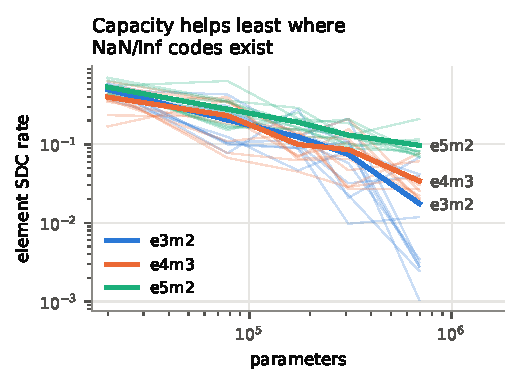
\includegraphics[width=0.62\linewidth]{figures/fig2_capacity.pdf}
\caption{Per-inference damage of an element fault against parameter count for ResNet8 at five
widths. Each faint line is one trained network; bold lines are means. Capacity helps least for
the format with the most NaN/Inf codes, and not at all for e5m2.}
\label{fig:capacity}
\end{figure}

\begin{figure}[htbp]
\centering
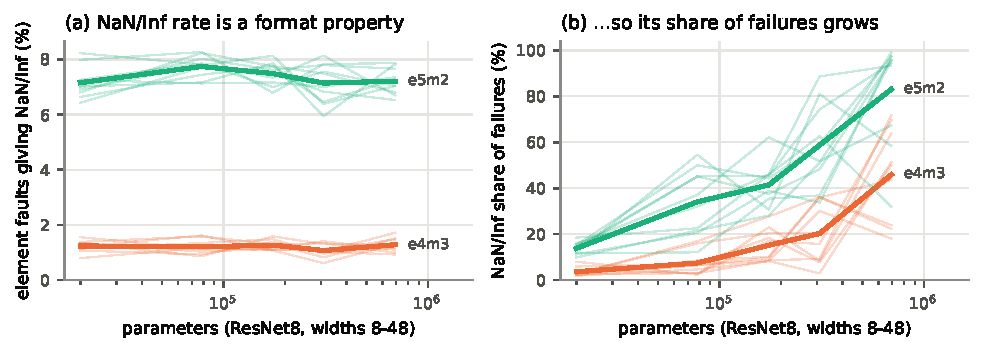
\includegraphics[width=\linewidth]{figures/fig22_nonfinite_width.pdf}
\caption{(a) The fraction of element faults that produce a non-finite output is flat across a
$35\times$ range of capacity. (b) Its share of all failures rises, because capacity absorbs
ordinary perturbations and never absorbs a NaN. e3m2 is zero everywhere and not drawn.}
\label{fig:nonfinite}
\end{figure}

\subsubsection{Second driver: the network's margin-normalised sensitivity}

Special codes cannot explain differences between formats that have none. On the ViT, e3m2 and
e2m3 are both 6-bit, both free of special codes and equally accurate, yet differed by
$5.8\times$ in element failures (Fisher exact $p=2.5\times10^{-30}$). I ruled out the size of the
perturbation (e2m3 actually perturbs weights \emph{less}, and still fails $7\times$ more often
within matched perturbation-size bins), which weights are hit, and differences in margin
distributions.

A probe with no bit patterns in it settled where the fragility lives: perturbing one random
weight by a fixed multiple of its layer's RMS separates the quantised networks completely. At
$1.5\times$ RMS, in 1500 trials, it never changed a prediction of the e3m2 or e5m2 networks, but
changed the e4m3 network's in $5\%$ of trials. The fragility is a property of the quantised
network, not of the encoding.

To explain it I defined a per-weight sensitivity
\[
s_i=\frac{|\partial m/\partial w_i|\cdot\mathrm{rms}}{m},
\]
where $m$ is the margin between the top two logits, maximised over evaluation images. A
perturbation of $\delta\cdot\mathrm{rms}$ should flip a prediction roughly when $s_i\delta>1$.
Computed by backpropagation, $s$ predicts the probe at correlation $+0.998$
(\fig{fig:sensitivity}a), and across all five formats it predicts the perturbation-driven
failure rate at $r=+0.93$, while mantissa width correlates at $-0.25$ (\fig{fig:sensitivity}b).
Among the 6- and 8-bit formats the 3-mantissa networks happen to be the more sensitive, but
e2m1, with the fewest mantissa bits and the highest sensitivity, shows that mantissa width is
not the cause.

\begin{figure}[htbp]
\centering
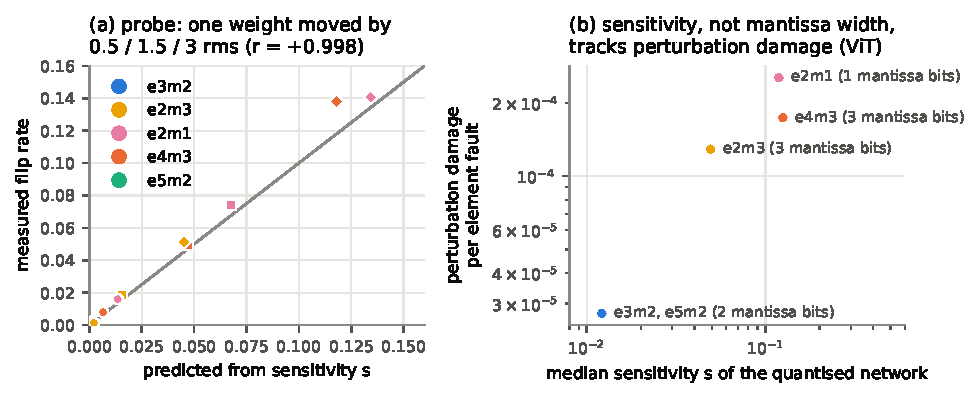
\includegraphics[width=\linewidth]{figures/fig21_sensitivity.pdf}
\caption{(a) The sensitivity $s$ predicts a format-agnostic probe (one weight moved by 0.5, 1.5
or 3 RMS; circles, squares, diamonds). (b) Across formats on the ViT, perturbation damage
follows the network's median sensitivity, not its mantissa width.}
\label{fig:sensitivity}
\end{figure}

\paragraph{What $s$ really measures.} Splitting $s$ into its two factors showed where the
difference between formats lies. The gradient factor agrees across all five formats to within
$1.08\times$; a permutation test that destroys any alignment between activations and gradients
moves the sensitivity tail by at most 2\%. The whole $10\times$ spread comes from the margin in
the denominator, and specifically from the \emph{one} evaluation image closest to a decision
boundary. That image belongs to the evaluation set, not to the network: $1/\min m$ ranks fifteen
networks by failure rate at Spearman $+0.98$ on the campaign's own 200 images but only $+0.21$ on
2000 fresh ones. Quantising to a different element format nudges the logits slightly, and
whether that nudge parks one of the evaluation images on a decision boundary is luck. This is
the same near-tie effect that \sect{sec:metricfind} identifies in the SDC metric.

\keybox{Two drivers. First, NaN/Inf element codes: they carry 97--100\% of element damage on
the larger networks, and capacity never absorbs them. Second, for the remaining perturbation
damage, the network's margin-normalised sensitivity ($r=+0.93$), not the format's mantissa or
exponent width.}

\subsection{A read-side guard for special codes}
\label{sec:guard}

If most element damage comes from one transition, into a special code, there is an obvious
defence: decode any special element code as zero when it is read. A fault that would have
produced NaN then only zeroes one weight. I tested this on all three architectures and both
datasets under e4m3 and e5m2. Every element fault that lands on a special code was found by
enumeration, so its share of the fault space is exact; a sample of 1000 of them was injected
with and without the guard, and 2000 other element faults (which the guard does not change)
once. The resulting estimate matched the exhaustive campaign to four significant figures
($0.016357\to0.003749$ against $0.016354\to0.003747$).

\begin{figure}[htbp]
\centering
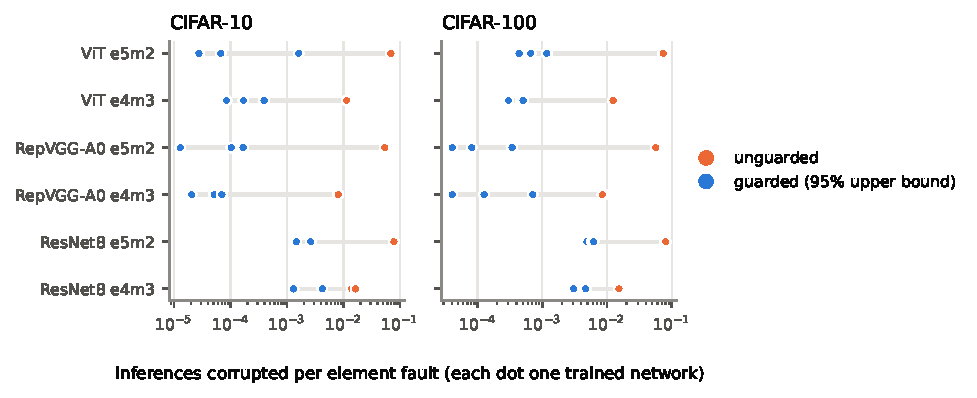
\includegraphics[width=\linewidth]{figures/fig18_nan_guard.pdf}
\caption{Per-inference damage of an element fault without (orange) and with (blue) the
read-side guard. The guarded value is a 95\% upper bound, since many guarded rates are zero in
the sample. Each dot is one trained network.}
\label{fig:guard}
\end{figure}

\begin{table}[htbp]
\centering\small
\caption{Effect of decoding special element codes as zero on read (CIFAR-10). The reduction is
the unguarded rate over a 95\% upper bound on the guarded rate, so it is a lower bound.}
\label{tab:guard}
\begin{tabular}{llcc}
\toprule
network & format & share of element damage from special codes & reduction, at least \\
\midrule
ResNet8 (2 nets)    & e4m3 & 78--93\%     & $3.9$--$10.7\times$ \\
ResNet8 (2 nets)    & e5m2 & 98--99\%     & $30$--$53\times$ \\
RepVGG-A0 (3 seeds) & e4m3 & 99.5--99.9\% & $115$--$389\times$ \\
RepVGG-A0 (3 seeds) & e5m2 & 99.9--100\%  & $319$--$4112\times$ \\
ViT (3 seeds)       & e4m3 & 97.1--99.5\% & $29$--$133\times$ \\
ViT (3 seeds)       & e5m2 & 99.9--100\%  & $43$--$2479\times$ \\
\bottomrule
\end{tabular}
\end{table}

On RepVGG and the ViT the guard cuts element damage by at least $29\times$ and up to
$4100\times$, bringing e5m2 down to the level of e3m2 (\fig{fig:guard}, \tab{tab:guard}). On
ResNet8 the reduction is smaller, because a small network is also fragile to ordinary
perturbations, which the guard does not touch. No guarded fault produced a non-finite output. On
CIFAR-100 the reductions are $13$--$1387\times$ on RepVGG and the ViT, smaller for the reason
given in \sect{sec:c100}. In hardware the guard is one comparator on the read path; I evaluated
it in software only.

\keybox{Decoding special element codes as zero on read removes nearly all element vulnerability
of e4m3 and e5m2 on the larger networks ($\ge29\times$, up to $4100\times$). It turns ``prefer
formats without special codes'' from a constraint into a choice.}

\subsection{CIFAR-100 as a harder task}
\label{sec:c100}

The natural target for the Transformer study is DeiT on ImageNet. ImageNet was not available
on the compute used for this study, so CIFAR-100 stands in for it: ten times the classes and a tenth of the
images per class, so networks sit much closer to their decision boundaries, which is the
property the margin results showed to matter. All three architectures were retrained with
unchanged recipes, three seeds each.

Every headline replicated. Formats were matched in accuracy (four formats within $0.01$ points on
the ViT), the ordering e3m2 $<$ e4m3 $<$ e5m2 held on all nine networks, scale faults outweighed
element faults everywhere ($1.7\times$ to $3600\times$), and NaN codes carried 94--100\% of e4m3
and e5m2 element damage on the larger networks.

What changed was the floor (\fig{fig:c100}, \tab{tab:c100}). With smaller margins, the formats
without special codes became $3$--$22\times$ more vulnerable, while e4m3 and e5m2 barely moved,
since a NaN corrupts an inference however wide the margins are. The gap between formats narrows:
on the ViT the e4m3/e3m2 ratio falls from $461\times$ to $19\times$. Among the NaN-free formats
the ordering does not carry over; on CIFAR-100 the ViT ranks e2m1 the safest of the three, which
is what the sensitivity result predicts.

\begin{figure}[htbp]
\centering
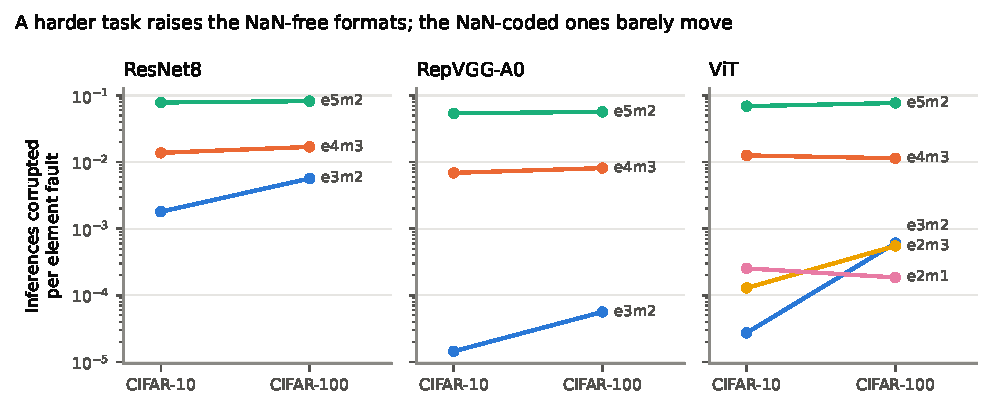
\includegraphics[width=\linewidth]{figures/fig20_cifar100.pdf}
\caption{Per-inference damage of an element fault on CIFAR-10 and CIFAR-100, mean over seeds.}
\label{fig:c100}
\end{figure}

\begin{table}[htbp]
\centering\small
\caption{Per-inference rate of element faults, CIFAR-10 $\rightarrow$ CIFAR-100, mean over
seeds.}
\label{tab:c100}
\begin{tabular}{lcccc}
\toprule
network & e3m2 (no special codes) & e4m3 & e5m2 & e4m3/e3m2 gap \\
\midrule
ViT       & $2.7\mathrm{e}{-5}\to6.1\mathrm{e}{-4}$ ($22\times$) & $0.0126\to0.0114$ & $0.069\to0.077$ & $461\times\to19\times$ \\
RepVGG-A0 & $1.4\mathrm{e}{-5}\to5.6\mathrm{e}{-5}$ ($3.9\times$) & $0.0069\to0.0081$ & $0.054\to0.057$ & $476\times\to144\times$ \\
ResNet8   & $1.8\mathrm{e}{-3}\to5.7\mathrm{e}{-3}$ ($3.2\times$) & $0.0137\to0.0169$ & $0.078\to0.082$ & $7.6\times\to3.0\times$ \\
\bottomrule
\end{tabular}
\end{table}

\keybox{Every result replicates on CIFAR-100. A harder task raises the perturbation floor of the
NaN-free formats and leaves the NaN pathway untouched, so the advantage of NaN-free formats is
smallest on exactly the harder tasks real deployments face.}

% =====================================================================
\section{Methodological findings}
\label{sec:methodfind}

Several findings concern how to measure MX reliability rather than MX reliability itself. They
apply to fault-injection studies in general.

\subsection{The any-image SDC metric measures the evaluation set}
\label{sec:metricfind}

The same 60 sign flips injected into the same width-32 ResNet8 move the logits by the same
amount under every format (median shift 0.12), yet change a prediction in 1 of 60 cases under
e4m3 and 26 of 60 under e3m2. The difference lies in the golden network: the e4m3 networks of
that width are the only ones of 39 with no evaluation image within 0.2 of a decision boundary.
Across all 39 width-sweep networks the any-image rate tracks the number of such near-tie images
at Spearman $+0.89$ (\fig{fig:neartie}). A near-tie image flips under almost any nudge, so one
of them can dominate a whole campaign.

\begin{figure}[htbp]
\centering
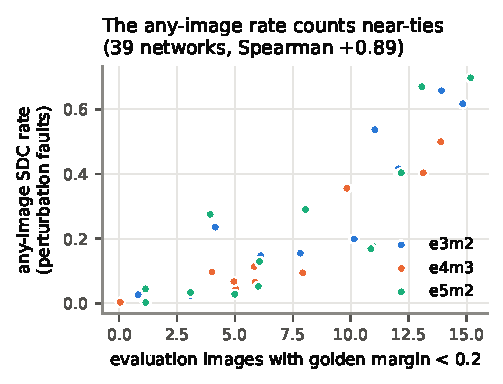
\includegraphics[width=0.55\linewidth]{figures/fig14_near_ties.pdf}
\caption{Any-image SDC rate of perturbation-driven element faults against the number of
evaluation images whose golden top-1/top-2 margin is below 0.2, for 39 width-sweep networks.}
\label{fig:neartie}
\end{figure}

To measure the effect directly, one fixed list of 1500 element faults per format was replayed against
nine disjoint, class-balanced sets of 200 images, on each of two networks
(\fig{fig:evalsets}). Under the any-image metric, e3m2 and e4m3 looked equal ($1.03\times$ and
$0.93\times$), their order reversed from one image set to the next, and the rate moved by up to
seven times its own confidence-interval width between sets, tracking each set's smallest margin
(Spearman $+0.80$ to $+0.93$). Scored per inference, the same faults on the same image sets gave
$5.6\times$ and $7.6\times$ between the formats, stable to within $1.15$--$1.27\times$ across
image sets.

\begin{figure}[htbp]
\centering
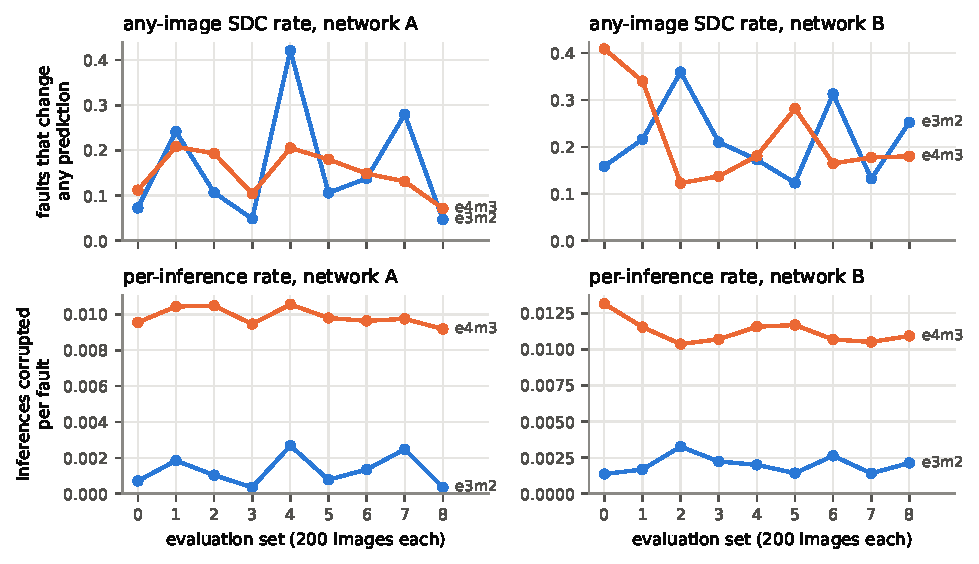
\includegraphics[width=\linewidth]{figures/fig13_eval_sets.pdf}
\caption{One fixed fault list per format replayed against nine evaluation sets, on two
independently trained ResNet8 networks. Top: the any-image rate makes the formats look equal and
reverses their order between sets. Bottom: the per-inference rate separates them consistently.}
\label{fig:evalsets}
\end{figure}

The any-image metric saturates: beyond a few dozen images it mostly reports whether the set
contains a near-tie input. The Wilson interval is not wrong, but it covers only the uncertainty
from sampling faults, while the choice of evaluation images is a second and larger source that
no number of injections reduces. Across all 119 weight campaigns the format ordering of
\tab{tab:formats-result} holds on 8 of 8 configurations per inference but on only 3 of 8 under
the any-image metric, which would wrongly suggest that the ranking of formats depends on the
architecture.

\subsection{Replicate over trained networks, not only over injections}

Two networks of the same architecture and width, differing only in their training seed, differed
in failure rate by a median of $12.8\times$ the uncertainty from 3000 injections. More
injections cannot reduce this spread; only more trained networks can. The capacity result of
\sect{sec:drivers} is therefore established with ten seeds per width and a slope test that
compares formats within each network. A result quoted from one trained network is much less
certain than its confidence interval suggests.

\subsection{A severity measure that predicts failure}
\label{sec:severity}

The log-ratio severity $d=|\log v'-\log v|$ does not predict failure: over 8374 element faults
on ResNet8 its rank correlation with observed failure is $0.026$. The reason is in the definition:
negating a value leaves $|v|$ unchanged, so a sign flip scores zero severity, although the sign
bit does the most finite damage of any bit. A sampler built on $d$ would give the most dangerous
perturbation bit almost no budget. Using the sensitivity of \sect{sec:drivers}, define
\[
\mathrm{margin\_shift}_i = s_i\,\frac{|v_i'-v_i|}{\mathrm{rms}},
\]
the fraction of the decision margin a fault consumes. Over $39{,}337$ finite element faults on
the ViT, $d$ reaches AUC $0.435$, slightly worse than chance, while $\mathrm{margin\_shift}$
reaches $0.990$ (\fig{fig:severity}, \tab{tab:severity}). Its natural threshold needs no tuning:
flagging faults with $\mathrm{margin\_shift}>1$ catches $98.5\%$ of all failures while flagging
only $4.4\%$ of the fault space.

\begin{figure}[htbp]
\centering
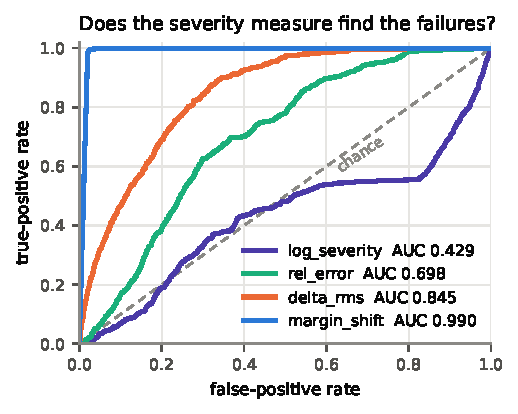
\includegraphics[width=0.55\linewidth]{figures/fig4_severity.pdf}
\caption{How well each severity measure ranks the faults that actually failed (ViT, finite
element faults). The log-ratio measure falls below the chance diagonal.}
\label{fig:severity}
\end{figure}

\begin{table}[htbp]
\centering\small
\caption{Severity measures against observed failure ($39{,}337$ finite element faults, ViT).}
\label{tab:severity}
\begin{tabular}{lccl}
\toprule
measure & Spearman & AUC & what it knows \\
\midrule
$|\log_2|v'|-\log_2|v||$ (log-ratio $d$) & $-0.035$ & 0.435 & number system only \\
$|v'-v|/|v|$ (relative error) & 0.107 & 0.699 & number system only \\
$|v'-v|/\mathrm{rms}$ & 0.184 & 0.845 & number system and layer scale \\
$\mathrm{margin\_shift}$ & 0.261 & \textbf{0.990} & number system and network \\
\bottomrule
\end{tabular}
\end{table}

\subsection{Value-aware sampling}
\label{sec:sampling}

\paragraph{Stratifying by site and layer.} With uniform sampling, a 3000-fault campaign draws
only about 100 scale faults. Neyman allocation with a blast-radius weight $\Phi$ moves 36\% of
the budget to scale bits and cuts the scale-stratum variance $10.5\times$, but widens the
model-wide interval: a trade between which estimate is precise, not a free gain. Plain
stratification by layer and site gives $0.94\times$, because per-layer failure rates are too
similar for Neyman allocation to exploit. The variance lives within the value distribution, not
across layers.

\paragraph{The target is zero-inflated.} The exhaustive campaigns show what the per-inference
target looks like (\fig{fig:zeroinfl}). Under e3m2, $92\%$ of element faults corrupt no inference
at all ($89\%$ of all faults); under e4m3, $60\%$. Almost all the variance sits in a thin tail, and
in e4m3 that tail includes a spike of faults that corrupt every inference, which are the flips
into NaN.

\begin{figure}[htbp]
\centering
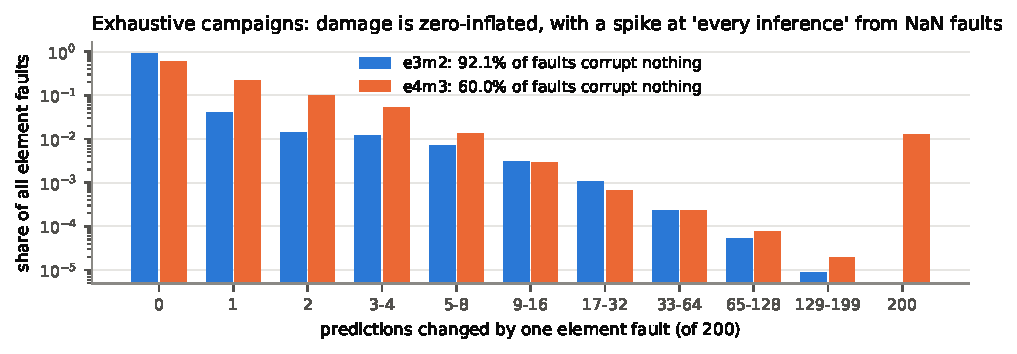
\includegraphics[width=\linewidth]{figures/fig15_zero_inflation.pdf}
\caption{Distribution of the number of predictions (of 200) changed by one element fault, over
every element fault of the two exhaustive ResNet8 campaigns. Logarithmic vertical axis.}
\label{fig:zeroinfl}
\end{figure}

\paragraph{Quantile strata.} The whole fault space is scored with $\mathrm{margin\_shift}$,
which costs only gradients, and cut into six strata at its 50th, 75th, 90th, 97th and 99.5th
percentiles; a fifth of the budget goes to a pilot that estimates each stratum's standard
deviation, and the rest is allocated by Neyman allocation. Replayed hundreds of times against both
exhaustive campaigns, variance fell $57$--$120\times$ against uniform sampling on both formats,
with no measurable bias (\fig{fig:sampling}). A 3000-injection stratified campaign is as precise
as a uniform one of $171{,}000$ (e4m3) to $346{,}000$ (e3m2) injections.

\begin{figure}[htbp]
\centering
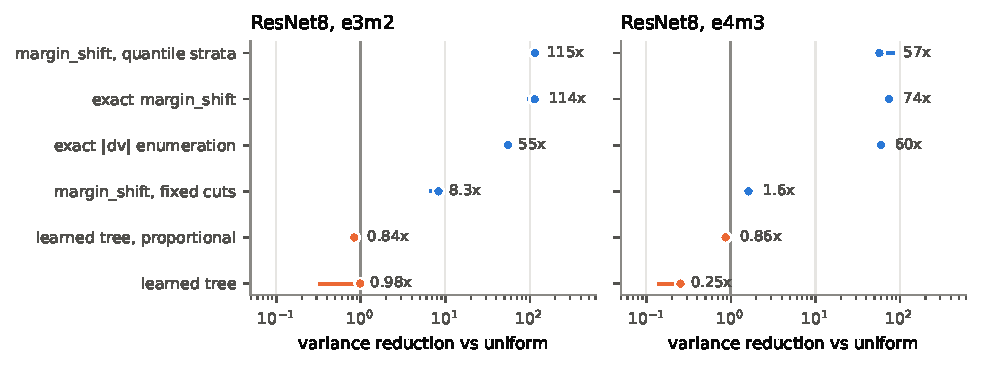
\includegraphics[width=\linewidth]{figures/fig16_sampling.pdf}
\caption{Variance reduction against uniform sampling for the per-inference rate, replayed
against exhaustive ground truth. Dots are at a budget of 3000 injections; bars span budgets of
500 to 3000. Orange arms do worse than uniform.}
\label{fig:sampling}
\end{figure}

\paragraph{Learned intervals versus exact enumeration.} Fault impact can be characterised as
TreeFI does, with value intervals learned by a regression tree from a
pilot, or by exact enumeration over the MX code table. Strata built from the exact $|v'-v|$
alone, with no gradient and no injections, cut variance $48$--$65\times$. Strata learned from a
20\% pilot never beat uniform sampling ($0.10$--$0.98\times$), at 6 or 16 leaves, with or without
the layer as a feature. Two things defeat the learner. A pilot of a few hundred faults, on a
target where most faults do nothing, sees too few failures to place its strata. And in e4m3 the
damaging tail is not a range of values at all: it is the discrete set of (code, bit) pairs that
land on NaN, which a code table lists exactly. Interval learning solves a problem FP32 has, an
alphabet of $2^{32}$ values, which MX does not.

\keybox{For MX formats, characterise fault impact by exact per-code enumeration ($48$--$65\times$),
optionally weighted by gradient sensitivity ($57$--$120\times$). Learned value intervals cost pilot
injections and return less than uniform sampling.}

\subsection{Single-bit versus multi-bit faults}
\label{sec:multibit}

To test whether multi-bit upsets need their own campaigns, 2000 stored words per format were
sampled on each of two ResNet8 networks and \emph{every} single- and double-bit pattern of each
word was injected, $390{,}000$ injections in all, recording which predictions changed. A random double flip in one word corrupts
$1.04$--$1.55\times$ as many inferences as a single flip, and an adjacent pair, the pattern a
multi-cell upset produces, $0.85$--$1.13\times$ (\fig{fig:multibit}a). The format ordering and
scale dominance are unchanged. Doubles are sub-additive, partly because a second flip can move a
word \emph{off} the NaN code its partner would have reached, and partly because two scale bits of
opposite value cancel.

Plugging the measured rates into the H-model expansion of \sect{sec:background}, doubles within a word reach
1\% of the expected damage only at a per-bit flip probability of $2$--$3\times10^{-3}$
(\fig{fig:multibit}b). At that rate ResNet8 already holds more than a thousand flipped bits at
once, so the one-fault-per-inference assumption that every campaign rests on fails through
accumulation across words about three orders of magnitude in $p$ before multiplicity within a word
matters.

\begin{figure}[htbp]
\centering
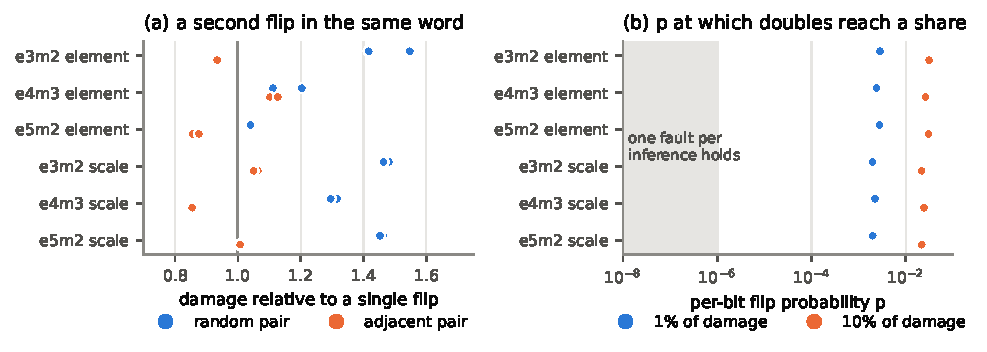
\includegraphics[width=\linewidth]{figures/fig17_multibit.pdf}
\caption{(a) Damage of a double flip in one word relative to a single flip, two networks per
row. (b) Per-bit flip probability at which within-word doubles reach 1\% and 10\% of expected
damage. The grey band marks where one fault per inference is a valid assumption.}
\label{fig:multibit}
\end{figure}

\keybox{Single-bit injection is sufficient. Within-word multi-bit upsets are a second-order
correction that only matters far beyond the regime where any single-fault campaign is valid.}

% =====================================================================
\section{Discussion}
\label{sec:discussion}

\subsection{Where the objectives stand}

\tab{tab:objectives} answers each objective, and \tab{tab:outcomes} sets the expected
outcomes against what was found.

\begin{table}[htbp]
\centering\small
\caption{The five objectives and their answers. All rates are per inference.}
\label{tab:objectives}
\begin{tabular}{@{}L{0.2\linewidth}L{0.75\linewidth}@{}}
\toprule
objective & answer \\
\midrule
O1 Fault propagation & A scale fault is always more damaging than an element fault, typically
$13\times$ to over $1000\times$, on every architecture, format, tensor type and dataset; less only
for e5m2 ($1.7$--$2.6\times$), whose element faults are already NaN-dominated. Scale faults also
produce non-finite outputs in 7--13\% of cases for every format. \\
O2 Format sensitivity & Formats of equal accuracy differ by up to three orders of magnitude.
e3m2 $<$ e4m3 $<$ e5m2 on all 8 CIFAR-10 configurations and all 9 CIFAR-100 networks. \\
O3 Block size & Larger blocks shrink the scale's share of storage ($11.1\%\to1.7\%$) but make each
scale fault worse, while element faults become milder. A genuine trade; with protected scales,
large blocks are safe. \\
O4 Tensor and location & Per fault, weights and activations are about equally dangerous
($0.3$--$2.2\times$); they differ in exposure. Among finite faults the sign bit is the worst
element bit, but flips into NaN dominate total damage. Scale flips that grow the block are
catastrophic. The small stem layer is the most fragile. \\
O5 Vulnerability drivers & First, NaN/Inf codes: they carry 97--100\% of element damage on the
larger models, and capacity cannot absorb them. Second, for the remaining perturbation damage,
the network's margin-normalised sensitivity ($r=+0.93$), not mantissa or exponent width. \\
\bottomrule
\end{tabular}
\end{table}

\begin{table}[htbp]
\centering\small
\caption{Expected outcomes against what was found.}
\label{tab:outcomes}
\begin{tabular}{@{}L{0.38\linewidth}L{0.57\linewidth}@{}}
\toprule
expected outcome & what was found \\
\midrule
Shared-scale faults have a significantly different, typically larger, impact & Confirmed
everywhere; never reversed on any model, format or dataset. \\
Reliability varies across formats at comparable accuracy & Confirmed, by up to three orders of
magnitude; explained by special codes and network sensitivity. \\
A block-size trade-off & Confirmed, with the two fault sites moving in opposite directions. \\
Per-tensor and per-location maps & Exhaustive per-bit and per-layer maps for ResNet8;
weight/activation comparison on six models. \\
Design guidance & \sect{sec:guidance}, including a read-side guard. \\
Open choice: learned vs.\ exact intervals & Settled: exact enumeration, $48$--$65\times$ against
$\le1\times$. \\
Open choice: single vs.\ multi-bit & Settled: single-bit is sufficient. \\
Open choice: the grid actually swept & All five formats and all four block sizes on CIFAR;
DeiT/ImageNet replaced by a ViT on CIFAR-100 (\sect{sec:limitations}). \\
\bottomrule
\end{tabular}
\end{table}

% =====================================================================
\section{Design guidance}
\label{sec:guidance}

\paragraph{For designers of MX accelerators.}
\begin{enumerate}
\item \textbf{Protect the shared scale first.} A scale fault typically does $13\times$ to more
than $1000\times$ the damage of an element fault, and scales are only 2--11\% of storage. Parity
or ECC on scale bytes is the cheapest protection with the largest payoff. If only some scale bits
can be protected, protect those normally at 0, whose flips grow the block.
\item \textbf{Neutralise special codes.} Prefer element formats without NaN/Inf codes, or decode
special element codes as zero on read. The guard removes most of the element vulnerability of
e4m3 and e5m2 on the larger models at the cost of one comparator.
\item \textbf{Do not judge reliability by accuracy or bit width.} Formats of equal accuracy
differ by orders of magnitude, and among NaN-free formats the ranking depends on the network and
task.
\item \textbf{Treat block size as a trade-off.} Larger blocks save scale storage but make each
scale fault worse. With protected scales, large blocks are safe.
\item \textbf{Prioritise early layers.} The small stem layer is the most fragile; protection
should follow vulnerability, not storage size.
\item \textbf{Size protection for weights and activations by exposure.} Per fault they are
equally dangerous; what differs is how long each word is resident and how often it is read.
\end{enumerate}

\paragraph{For anyone running fault-injection campaigns on MX models.}
\begin{enumerate}[resume]
\item Report the per-inference rate, not the any-image SDC rate.
\item Replicate over several independently trained networks.
\item Inject single-bit faults; double-bit faults add no first-order information.
\item Stratify by exact per-code enumeration of the decoded change, weighted by gradient
sensitivity where available, for $57$--$120\times$ fewer injections at the same precision.
\item Tie every campaign to its exact checkpoint, and verify it by replaying recorded faults.
\item Run the deployment form of the network: fold batch norm and fuse branches before
quantising.
\end{enumerate}

% =====================================================================
\section{Limitations and future work}
\label{sec:limitations}

\paragraph{ImageNet and DeiT were not evaluated.} ImageNet was not reachable from any machine
available to me, so CIFAR-100 stood in for it, with a small vision Transformer trained from
scratch at DeiT-Tiny width. That network reaches only 47--49\% on CIFAR-100, far below a
pretrained DeiT on ImageNet. The CIFAR-100 study shows that the conclusions survive a harder task
with smaller margins; it is not a measurement of DeiT on ImageNet. The trend it reveals, a
narrowing gap between formats as margins shrink, suggests that absolute gaps at ImageNet scale
may be smaller than on CIFAR-10. The directions of the effects, which held on every network, are
the more transferable result.

\paragraph{Model scale.} The largest network has 7 million parameters. The optional small LLM
and MXINT8 were not studied. The capacity results suggest that larger models absorb perturbations
but not NaNs, which would make special codes even more dominant, but I did not test this
directly.

\paragraph{Fault model.} Only faults in stored values are modelled: weights, activations and
their scales. Datapath, accumulator, control and timing faults are out of scope. Every stored bit
is assumed equally likely to flip ($\kappa\equiv1$); a graded profile
would reweight the per-bit results but not change them.

\paragraph{Other.} Campaigns score a fixed subset of 200 images (100 for activations) to keep
millions of injections affordable. The per-inference rate is robust to this choice, but absolute
rates carry the uncertainty of the subset. The NaN guard was evaluated in software, not in
hardware, and the mechanism behind the element-side block-size trend is not established.

\paragraph{Future work.} The most useful next step is to repeat the key campaigns (format
ordering, scale dominance, the NaN guard) on a pretrained Transformer at ImageNet scale and on a
small language model. A hardware model of the guard, and a protection scheme that combines
scale ECC with the guard and is costed in area and energy, would turn the guidance into a
design.

% =====================================================================
\section{Conclusion}
\label{sec:conclusion}

This work asked whether the reliability of microscaling DNNs varies across formats at comparable
accuracy, and whether faults in the shared scale behave differently from faults in elements.
Both answers are yes, on every network I tested. Formats of equal accuracy differ by up to three
orders of magnitude, and a scale fault is always more damaging than an element fault, typically
by $13\times$ to more than $1000\times$.

The study also found out why. Most element damage comes from the small fraction of flips that
land on NaN or infinity codes. No amount of model capacity absorbs them, and a simple read-side
guard removes them. What is left is governed by the decision margins of the network, not by how
many mantissa bits the format has.

The work also contributes a bit-accurate fault-injection library validated against exhaustive
ground truth, shows that the conventional SDC metric can hide the differences it is meant to
reveal, gives a severity measure that predicts failure and cuts campaign cost by two orders of
magnitude, and settles both open design choices of the methodology.

\paragraph{Code and data.} The \texttt{mxfi} library, every experiment script, the trained
networks and the raw campaign outputs are in the project repository
(\url{https://github.com/peeyushagarwal2004/CS496_UGP}). The complete experiment log is
in \texttt{docs/findings.md}.

\paragraph{Acknowledgements.} I am grateful to my supervisor for the problem statement and for
guidance throughout, and to IIT Kanpur for access to the GPU server on which most of the later
experiments ran.

% =====================================================================
\begin{thebibliography}{99}
\small
\addcontentsline{toc}{section}{References}

\bibitem{rouhani2023mx}
B.~D. Rouhani et al., ``Microscaling data formats for deep learning,''
\emph{arXiv:2310.10537}, 2023.

\bibitem{ocp2023mx}
Open Compute Project, ``OCP Microscaling Formats (MX) Specification, Version 1.0,'' 2023.

\bibitem{li2017understanding}
G.~Li, S.~K.~S. Hari, M.~Sullivan, T.~Tsai, K.~Pattabiraman, J.~Emer, and S.~W. Keckler,
``Understanding error propagation in deep learning neural network (DNN) accelerators and
applications,'' in \emph{Proc. SC}, 2017.

\bibitem{reagen2018ares}
B.~Reagen et al., ``Ares: A framework for quantifying the resilience of deep neural
networks,'' in \emph{Proc. DAC}, 2018.

\bibitem{mahmoud2020pytorchfi}
A.~Mahmoud et al., ``PyTorchFI: A runtime perturbation tool for DNNs,'' in \emph{Proc.
DSN Workshops}, 2020.

\bibitem{hong2019terminal}
S.~Hong, P.~Frigo, Y.~Kaya, C.~Giuffrida, and T.~Dumitra\c{s}, ``Terminal brain damage:
Exposing the graceless degradation in deep neural networks under hardware fault attacks,''
in \emph{Proc. USENIX Security}, 2019.

\bibitem{rakin2019bfa}
A.~S. Rakin, Z.~He, and D.~Fan, ``Bit-flip attack: Crushing neural network with progressive
bit search,'' in \emph{Proc. ICCV}, 2019.

\bibitem{leveugle2009sfi}
R.~Leveugle, A.~Calvez, P.~Maistri, and P.~Vanhauwaert, ``Statistical fault injection:
Quantified error and confidence,'' in \emph{Proc. DATE}, 2009.

\bibitem{treefi2026}
TreeFI: value-aware statistical fault injection for DNNs, in \emph{Proc. ICCAD}, 2026.

\bibitem{he2016resnet}
K.~He, X.~Zhang, S.~Ren, and J.~Sun, ``Deep residual learning for image recognition,'' in
\emph{Proc. CVPR}, 2016.

\bibitem{banbury2021mlperftiny}
C.~Banbury et al., ``MLPerf Tiny benchmark,'' in \emph{Proc. NeurIPS Datasets and
Benchmarks Track}, 2021.

\bibitem{ding2021repvgg}
X.~Ding, X.~Zhang, N.~Ma, J.~Han, G.~Ding, and J.~Sun, ``RepVGG: Making VGG-style ConvNets
great again,'' in \emph{Proc. CVPR}, 2021.

\bibitem{dosovitskiy2021vit}
A.~Dosovitskiy et al., ``An image is worth 16x16 words: Transformers for image recognition
at scale,'' in \emph{Proc. ICLR}, 2021.

\bibitem{touvron2021deit}
H.~Touvron, M.~Cord, M.~Douze, F.~Massa, A.~Sablayrolles, and H.~J\'egou, ``Training
data-efficient image transformers \& distillation through attention,'' in \emph{Proc.
ICML}, 2021.

\bibitem{wilson1927}
E.~B. Wilson, ``Probable inference, the law of succession, and statistical inference,''
\emph{J. American Statistical Association}, vol.~22, 1927.

\bibitem{neyman1934}
J.~Neyman, ``On the two different aspects of the representative method,'' \emph{J. Royal
Statistical Society}, vol.~97, 1934.

\end{thebibliography}

% =====================================================================
\clearpage
\appendix

\section{Experiment index}
\label{app:experiments}

Every experiment is a script in \texttt{experiments/}; its docstring says what it tests and how to
run it. Raw outputs are in \texttt{results/} (CPU runs) and \texttt{cluster/results/} (GPU
runs).

\begin{longtable}{@{}lL{0.40\linewidth}L{0.38\linewidth}@{}}
\caption{Experiments and the findings they support.}\label{tab:experiments}\\
\toprule
script & question & used in \\
\midrule
\endfirsthead
\toprule
script & question & used in \\
\midrule
\endhead
\texttt{e00} & Quantised accuracy for every format, block size and scale rule & \fig{fig:accuracy} \\
\texttt{e01} & Uniform 3000-fault weight campaign for one cell of the grid & Sections~\ref{sec:formats}, \ref{sec:sites} \\
\texttt{e02} & Uniform versus Neyman versus Neyman-with-$\Phi$ allocation & \sect{sec:sampling} \\
\texttt{e03}, \texttt{e03b} & Block size; matched faults under OCP and fit & \sect{sec:blocksize} \\
\texttt{e04} & Activation faults & \sect{sec:act} \\
\texttt{e05c} & Near-tie images and tie-robust metrics & \sect{sec:metricfind} \\
width sweeps & ResNet8 at five widths, up to ten seeds & \sect{sec:drivers} \\
\texttt{e06} & Exhaustive campaigns & Sections~\ref{sec:groundtruth}, \ref{sec:location} \\
\texttt{e08}--\texttt{e10} & Format geometry, perturbation size against damage, margins & \sect{sec:drivers} \\
\texttt{e11} & Per-weight sensitivity and the format-agnostic probe & \fig{fig:sensitivity} \\
\texttt{e12} & Severity measures against observed failure & \sect{sec:severity} \\
\texttt{e14}, \texttt{e16} & Origin of the sensitivity tail; alignment permutation test & \sect{sec:drivers} \\
\texttt{e15} & Value-aware sampling, any-image rate & \sect{sec:sampling} \\
\texttt{e17}, \texttt{e18} & Near-tie screen; one fault list on nine evaluation sets & \sect{sec:metricfind} \\
\texttt{e19} & Every campaign rescored per inference & \sect{sec:results} \\
\texttt{e20} & Value-aware sampling, per-inference rate & \sect{sec:sampling} \\
\texttt{e21} & Single- versus double-bit faults & \sect{sec:multibit} \\
\texttt{e22} & Learned value intervals versus exact enumeration & \sect{sec:sampling} \\
\texttt{e23} & Read-side NaN guard & \sect{sec:guard} \\
\texttt{e24} & CIFAR-100 against CIFAR-10 & \sect{sec:c100} \\
\bottomrule
\end{longtable}

\section{Reproducing the results}
\label{app:repro}

The repository tracks the code, every raw campaign output, the trained networks and the CIFAR
datasets (the three largest files through Git LFS). With Python 3.11 or later:

\begin{verbatim}
python -m venv .venv
.venv/Scripts/python -m pip install -r requirements.txt \
    --extra-index-url https://download.pytorch.org/whl/cpu
.venv/Scripts/python -m pytest tests -q            # 214 tests

python -m mxfi.train --model resnet8 --epochs 60
python -m experiments.e01_uniform_baseline --model resnet8 --fmt e4m3
python -m experiments.make_figures          # four core figures
python -m experiments.make_report_figures   # all other figures
\end{verbatim}

\noindent Set \texttt{PYTHONPATH=.} when running from the repository root. A model name ending
in \texttt{\_c100} trains and evaluates on CIFAR-100. The heavier runs used \texttt{--device
cuda} on an A100. \texttt{cluster/} is a verbatim mirror of the GPU server's checkpoints,
results and logs, kept separate from the CPU runs because same-named checkpoints on the two
machines hold different weights.

\end{document}
